% !TEX program = pdflatex
\documentclass[11pt, a4paper]{article}

% ──────────────────────────── Packages ────────────────────────────
\usepackage[utf8]{inputenc}
\usepackage[T1]{fontenc}
\usepackage{lmodern}
\usepackage[margin=2.2cm]{geometry}
\usepackage{amsmath, amssymb}
\usepackage{booktabs}
\usepackage{graphicx}
\usepackage{xcolor}
\usepackage{hyperref}
\usepackage{cleveref}
\usepackage{caption, subcaption}
\usepackage{float}
\usepackage{enumitem}
\usepackage{multirow}
\usepackage{array}
\usepackage{tabularx}
\usepackage{pgfplots}
\pgfplotsset{compat=1.18}
\usepgfplotslibrary{groupplots}
\usepackage{algorithm}
\usepackage{algpseudocode}
% Bibliography handled via thebibliography (no biber required)

\hypersetup{
  colorlinks=true,
  linkcolor=blue!60!black,
  citecolor=green!50!black,
  urlcolor=blue!70!black,
}

\graphicspath{{report_figures/}}

% ──────────────────────── Custom Commands ─────────────────────────
\newcommand{\map}{\text{mAP}}
\newcommand{\mapfifty}{\text{mAP}_{50}}
\newcommand{\mapfull}{\text{mAP}_{50\text{-}95}}
\newcommand{\yolobase}{\textsc{Yolo26s}}
\newcommand{\yolop}{\textsc{Yolo26s-P2}}

% No external bib file needed

% ═══════════════════════════════════════════════════════════════════
\begin{document}

% ──────────────────────────── Title ───────────────────────────────
\title{%
  \textbf{Multi-Stage Training Strategy for Small Rocket Detection\\
    with YOLO26s-P2 and COCO Hard Negative Mining}}
\author{%
  Training Report --- ROCAM Small Object Detection Pipeline
}
\date{March 2026}
\maketitle

% ──────────────────────────── Abstract ────────────────────────────
\begin{abstract}
  We present a systematic, multi-stage training pipeline for detecting
  small rockets in surveillance imagery captured by the ROCAM system.
  Starting from a vanilla \yolobase{} baseline
  ($\mapfull = 0.694$), we upgrade to the \yolop{} architecture---which
  adds a stride-4 detection head tailored for small targets---and
  introduce COCO hard negative mining to suppress false positives.
  Although the architectural change and harder training distribution
  initially \emph{degrade} $\mapfull$ to $0.614$ ($-11.5\%$), a
  carefully designed three-stage fine-tuning protocol progressively
  recovers and surpasses the baseline, achieving a final
  $\mapfull = 0.750$ ($+8.1\%$ over the original) and
  $\mapfifty = 0.958$.  All experiments are conducted on a
  $4{\times}$NVIDIA H100~PCIe cluster using Distributed Data Parallel
  (DDP) training with mixed precision.  We analyse each stage's
  contribution, discuss failure modes encountered during the process,
  and provide actionable insights for practitioners training small-object
  detectors.
\end{abstract}

% ═══════════════════════════════════════════════════════════════════
\section{Introduction}
\label{sec:intro}

Detecting small, fast-moving rockets in surveillance footage poses unique
challenges for modern object detectors. The targets of interest typically
occupy fewer than $30{\times}30$ pixels in $960{\times}544$ frames, can appear
at \emph{any} orientation ($0$--$360^{\circ}$), and are subject to imaging
degradation including motion blur, compression artefacts, and varying
illumination.

The YOLO family of detectors~\cite{ultralytics2025yolo} offers an attractive
balance between speed and accuracy for real-time deployment. However, vanilla
YOLO architectures are optimised for objects at strides $\{8, 16, 32\}$, which
may miss very small targets. The \textbf{P2 variant} introduces an additional
detection head at stride~$4$, quadrupling the spatial resolution of the finest
feature map.

In this report we document the complete training journey---from an initial
\yolobase{} baseline through architecture upgrade, data engineering (COCO hard
negative mining), and a three-stage fine-tuning protocol. Our contributions
are:

\begin{enumerate}[leftmargin=*]
  \item \textbf{Architecture upgrade}: adoption of \yolop{} with a
        stride-4 detection head, increasing small-target sensitivity
        at a modest $+22\%$ GFLOPs cost.
  \item \textbf{COCO hard negative mining}: automated injection of
        4{,}000 background images from MS~COCO~\cite{lin2014coco} to
        suppress false positives, constituting $\sim\!25\%$ of the
        training set.
  \item \textbf{Multi-stage fine-tuning}: a three-stage protocol
        (close-mosaic, ultra-fine polish) that recovers the
        performance drop caused by the harder training distribution
        and pushes $\mapfull$ from $0.614$ to $0.750$.
  \item \textbf{Failure analysis}: documentation of two failed
        fine-tuning attempts and the lessons learned (optimizer
        pitfalls, learning-rate scheduling).
\end{enumerate}

% ═══════════════════════════════════════════════════════════════════
\section{Dataset}
\label{sec:dataset}

\subsection{ROCAM Dataset}

The ROCAM dataset is a single-class (\texttt{rocket}) object detection dataset
derived from surveillance camera footage. Key statistics are summarised
in~\Cref{tab:dataset}.

\begin{table}[h]
  \centering
  \caption{ROCAM dataset statistics.}
  \label{tab:dataset}
  \begin{tabular}{@{}lrrr@{}}
    \toprule
    \textbf{Split}     & \textbf{Images}   & \textbf{Resolution} & \textbf{Notes}             \\
    \midrule
    Train (original)   & 11{,}832          & $960{\times}544$    & Annotated rockets          \\
    Train (+ COCO neg) & 15{,}832          & mixed               & +4{,}000 background images \\
    Validation         & 3{,}378           & $960{\times}544$    &                            \\
    Test               & 3{,}421           & $960{\times}544$    &                            \\
    \midrule
    \textbf{Total}     & \textbf{22{,}631} &                     & Single class               \\
    \bottomrule
  \end{tabular}
\end{table}

Images are sourced from industrial surveillance cameras with a native
resolution of $960{\times}544$ (non-square, $\sim\!16{:}9$ aspect ratio).
Annotations follow the YOLO format (class, $x_c$, $y_c$, $w$, $h$ normalised to
$[0,1]$).

\subsection{COCO Hard Negative Mining}
\label{sec:coco_neg}

A persistent issue in small-object detection is the high false-positive rate:
the model learns to fire on textured background regions that resemble the
target at small scales. To address this, we inject \textbf{pure background
  images} from MS~COCO~\cite{lin2014coco} into the training set.

\begin{algorithm}[h]
  \caption{COCO Hard Negative Mining Pipeline}
  \label{alg:coco}
  \begin{algorithmic}[1]
    \Require COCO train2017 + val2017 images (${\sim}123$K total)
    \Require Target count $N = 4{,}000$
    \State Download and extract COCO images (cached after first run)
    \State $S \gets \textsc{RandomSample}(\text{all COCO images}, N, \text{seed}=0)$
    \For{each image $s_i \in S$}
    \State Copy $s_i$ to \texttt{images/train/coco\_neg\_\{i\}.jpg}
    \State Create empty label file \texttt{labels/train/coco\_neg\_\{i\}.txt}
    \EndFor
  \end{algorithmic}
\end{algorithm}

The empty label files ensure YOLO treats these images as containing \emph{zero}
objects, providing pure background supervision. At $N=4{,}000$, the negatives
constitute $\sim\!25.3\%$ of the training set---a ratio chosen through
iterative experimentation (see \Cref{sec:discussion}).

% ═══════════════════════════════════════════════════════════════════
\section{Model Architecture}
\label{sec:arch}

\subsection{YOLO26s Baseline}

YOLO26~\cite{ultralytics2025yolo} is the latest generation of the Ultralytics
YOLO family, featuring an updated backbone and a dual-head design (one-to-one
for end-to-end inference, one-to-many for higher-recall training). The
\textbf{small} variant (\yolobase) has ${\sim}10$M parameters and natively
detects at strides $\{8, 16, 32\}$.

\subsection{P2 Variant: Stride-4 Detection Head}

The \yolop{} variant adds a \textbf{P2 detection head} at stride~$4$, which
operates on a feature map with $4{\times}$ the spatial resolution of the
standard finest level. This is critical for our application where rocket
targets can be as small as $10{\times}10$~pixels.

\begin{table}[h]
  \centering
  \caption{Architecture comparison: \yolobase{} vs.\ \yolop{}.}
  \label{tab:arch}
  \begin{tabular}{@{}lccc@{}}
    \toprule
    \textbf{Model} & \textbf{Parameters} & \textbf{GFLOPs} & \textbf{Detection Strides} \\
    \midrule
    \yolobase{}    & ${\sim}10.0$M       & baseline        & $\{8, 16, 32\}$            \\
    \yolop{}       & ${\sim}9.8$M        & $+22\%$         & $\{4, 8, 16, 32\}$         \\
    \bottomrule
  \end{tabular}
\end{table}

Both variants use transfer learning from COCO-pretrained \texttt{yolo26s.pt}
weights, with matching layers automatically migrated to the P2 architecture.

% ═══════════════════════════════════════════════════════════════════
\section{Training Methodology}
\label{sec:method}

Our training pipeline consists of four distinct phases, as illustrated
in~\Cref{fig:pipeline}.

\begin{figure}[h]
  \centering
  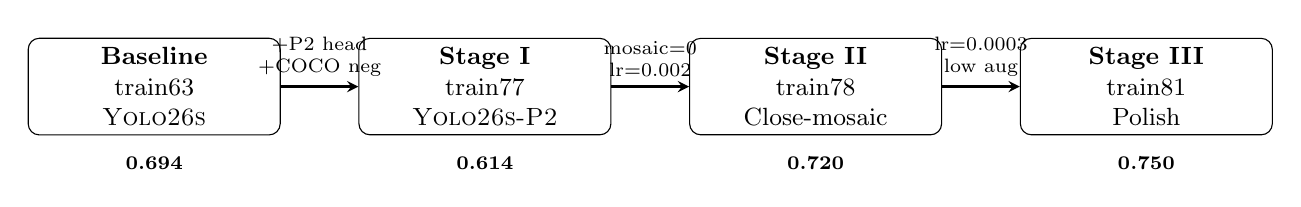
\begin{tikzpicture}[
      stage/.style={draw, rounded corners, minimum width=3.2cm,
          minimum height=1cm, align=center, font=\small},
      arrow/.style={->, thick, >=stealth},
      label/.style={font=\scriptsize, align=center}
    ]
    \node[stage] (s0) at (0,0) {\textbf{Baseline}\\train63\\\yolobase};
    \node[stage] (s1) at (4.2,0) {\textbf{Stage~I}\\train77\\\yolop};
    \node[stage] (s2) at (8.4,0) {\textbf{Stage~II}\\train78\\Close-mosaic};
    \node[stage] (s3) at (12.6,0) {\textbf{Stage~III}\\train81\\Polish};
    \draw[arrow] (s0) -- node[above, label] {+P2 head\\+COCO neg} (s1);
    \draw[arrow] (s1) -- node[above, label] {mosaic=0\\lr=0.002} (s2);
    \draw[arrow] (s2) -- node[above, label] {lr=0.0003\\low aug} (s3);
    \node[below=0.15cm, font=\scriptsize\bfseries] at (s0.south) {0.694};
    \node[below=0.15cm, font=\scriptsize\bfseries] at (s1.south) {0.614};
    \node[below=0.15cm, font=\scriptsize\bfseries] at (s2.south) {0.720};
    \node[below=0.15cm, font=\scriptsize\bfseries] at (s3.south) {0.750};
  \end{tikzpicture}
  \caption{Training pipeline overview.  Numbers below each stage
    indicate the best $\mapfull$ achieved. Note the initial
    \emph{decrease} after Stage~I, which is recovered through fine-tuning.}
  \label{fig:pipeline}
\end{figure}

% ── 4.1 Baseline ──
\subsection{Baseline: Vanilla YOLO26s (train63)}
\label{sec:baseline}

The baseline model uses the vanilla \yolobase{} architecture trained from
COCO-pretrained weights on a single GPU. Key configuration:

\begin{itemize}[leftmargin=*, itemsep=2pt]
  \item \textbf{Hardware}: 1$\times$ NVIDIA H100 PCIe (81\,GB)
  \item \textbf{Batch size}: 64, image size $[544, 960]$
  \item \textbf{Epochs}: 420 (all completed, no early stopping)
  \item \textbf{Scheduler}: linear decay, $\text{lr}_0 = 0.01$,
        $\text{lrf} = 0.01$
  \item \textbf{Augmentation}: aggressive---mosaic$=1.0$,
        cutmix$=0.1$, scale$=0.3$, close\_mosaic$=80$
  \item \textbf{COCO negatives}: none
\end{itemize}

\noindent\textbf{Result}: epoch~419, $\mapfifty = 0.948$,
$\mapfull = 0.694$.

% ── 4.2 Stage I ──
\subsection{Stage~I: P2 Architecture + COCO Negatives (train76/77)}
\label{sec:stage1}

Stage~I introduces two major changes simultaneously:

\begin{enumerate}[leftmargin=*]
  \item \textbf{Architecture}: upgrade from \yolobase{} to \yolop{}
        (\texttt{yolo26s-p2.yaml}), adding the stride-4 head.
  \item \textbf{Data}: inject COCO hard negatives (initially 1{,}000
        in train76, increased to 4{,}000 in train77).
\end{enumerate}

\noindent Augmentation is \emph{reduced} relative to the baseline to
protect small targets: mosaic $1.0 \to 0.8$, cutmix
$0.1 \to 0.0$, scale $0.3 \to 0.15$.

\begin{table}[h]
  \centering
  \caption{Stage~I configuration evolution.}
  \label{tab:stage1}
  \begin{tabular}{@{}lcc@{}}
    \toprule
    \textbf{Parameter} & \textbf{train76} & \textbf{train77} \\
    \midrule
    GPUs               & 3 (H100)         & 4 (H100)         \\
    COCO negatives     & 1{,}000          & 4{,}000          \\
    Patience           & 30               & 50               \\
    $\text{lrf}$       & 0.01             & 0.02             \\
    close\_mosaic      & 150              & 250              \\
    \midrule
    Best $\mapfull$    & 0.652 (ep335)    & 0.614 (ep267)    \\
    Epochs run         & 365/600          & 317/600          \\
    \bottomrule
  \end{tabular}
\end{table}

\paragraph{Critical issue.}  Both runs terminated via early stopping \emph{before} the
\texttt{close\_mosaic} epoch was reached. In train77 with close\_mosaic$=250$,
mosaic augmentation was scheduled to disable at epoch $600 - 250 = 350$, but
training stopped at epoch~317 (patience$=50$). Consequently, the model
\textbf{never trained on full-resolution images}---it only ever saw
$\frac{1}{4}$-scale mosaic composites, severely limiting small-target
localisation precision.

% ── 4.3 Stage II ──
\subsection{Stage~II: Close-Mosaic Fine-Tuning (train78)}
\label{sec:stage2}

To address the missed close-mosaic phase, we fine-tune from
\texttt{train77/best.pt} (epoch~267) with mosaic \emph{completely disabled}:

\begin{itemize}[leftmargin=*, itemsep=2pt]
  \item \textbf{Mosaic}$= 0.0$, \textbf{mixup}$= 0.0$, cutmix$= 0.0$
  \item $\text{lr}_0 = 0.002$ ($\frac{1}{5}$ of Stage~I),
        cosine schedule~\cite{loshchilov2016sgdr}, $\text{lrf} = 0.05$
  \item 5-epoch warmup to smooth the distribution shift
  \item 100 epochs, patience$= 40$
  \item Erasing reduced $0.4 \to 0.2$
\end{itemize}

\noindent\textbf{Result}: The model saw full-resolution
($960\times544$) images for the first time, and $\mapfull$ \textbf{jumped
  from $0.614$ to $0.720$} ($+17.3\%$), reaching
$\mapfifty = 0.955$.  This is the \textbf{single largest improvement}
in the entire pipeline.

% ── 4.4 Stage III ──
\subsection{Stage~III: Ultra-Fine Polish (train81)}
\label{sec:stage3}

The final stage applies a very low learning rate to ``polish'' the model into
its optimal basin:

\begin{itemize}[leftmargin=*, itemsep=2pt]
  \item Resume from \texttt{train78/best.pt} (epoch~93, $\mapfull = 0.720$)
  \item $\text{lr}_0 = 0.0003$ ($\frac{1}{7}$ of Stage~II),
        \textbf{SGD explicitly set} (not \texttt{auto})
  \item Cosine decay to $\text{lr}_0 \times 0.2 = 6 \times 10^{-5}$
  \item \texttt{multi\_scale = False}: fixed $960$\,px for deployment
        resolution
  \item Augmentation further reduced: scale $0.15 \to 0.08$, shear $5.0 \to 2.0$,
        translate $0.05 \to 0.02$
  \item Albumentations probabilities lowered by ${\sim}30\%$
  \item 60 epochs, patience$= 25$
\end{itemize}

\noindent\textbf{Result}: $\mapfull$ improved from $0.720$ to
$\mathbf{0.750}$ ($+4.2\%$), with $\mapfifty = 0.958$,
precision $= 0.961$, recall $= 0.915$.

% ── 4.5 Failed Attempts ──
\subsection{Failed Attempts and Lessons Learned}
\label{sec:failures}

\paragraph{train79 (1 epoch only).}  An attempt to fine-tune with \texttt{optimizer = ``auto''} and $\text{lr}_0 =
  0.0003$. Ultralytics' auto-optimizer selected AdamW and \emph{ignored} the
specified $\text{lr}_0$, applying its own scaling. The run was aborted after
one epoch upon discovering the unexpected learning rate.

\paragraph{train80 (no results).}  Fixed the optimizer to \texttt{SGD} but encountered a configuration issue that
prevented results from being saved.

\paragraph{Lesson.}  When fine-tuning with a specific learning rate, \textbf{always set the
  optimizer explicitly} (e.g., \texttt{optimizer=`SGD'}). The \texttt{auto} mode
applies internal heuristics that can override user-specified hyperparameters.

% ═══════════════════════════════════════════════════════════════════
\section{Data Augmentation Strategy}
\label{sec:augmentation}

A distinctive aspect of this pipeline is the \textbf{progressive reduction} of
augmentation intensity across stages, summarised in~\Cref{tab:augmentation}.

\begin{table}[h]
  \centering
  \caption{Augmentation parameters across training stages.  Values
    decrease from left to right, reflecting the shift from exploration
    (learning diverse features) to exploitation (precision refinement).}
  \label{tab:augmentation}
  \small
  \begin{tabular}{@{}lcccc@{}}
    \toprule
    \textbf{Parameter} & \textbf{Baseline} & \textbf{Stage~I} & \textbf{Stage~II} & \textbf{Stage~III} \\
                       & (train63)         & (train77)        & (train78)         & (train81)          \\
    \midrule
    mosaic             & 1.0               & 0.8              & 0.0               & 0.0                \\
    mixup              & 0.10              & 0.10             & 0.0               & 0.0                \\
    cutmix             & 0.10              & 0.0              & 0.0               & 0.0                \\
    scale              & 0.30              & 0.15             & 0.15              & 0.08               \\
    shear              & 5.0               & 5.0              & 5.0               & 2.0                \\
    translate          & 0.05              & 0.05             & 0.05              & 0.02               \\
    perspective        & 0.0002            & 0.0002           & 0.0002            & 0.0001             \\
    degrees            & 180               & 180              & 180               & 180                \\
    flipud             & 0.5               & 0.5              & 0.5               & 0.5                \\
    fliplr             & 0.5               & 0.5              & 0.5               & 0.5                \\
    erasing            & 0.4               & 0.4              & 0.2               & 0.05               \\
    hsv\_h / s / v     & .015/.6/.4        & .015/.6/.4       & .015/.6/.4        & .01/.4/.3          \\
    \bottomrule
  \end{tabular}
\end{table}

\paragraph{180$^{\circ}$ rotation.}  Full rotation is retained across
\emph{all} stages because rockets in flight can appear at any
orientation---this augmentation matches the true data distribution.

\paragraph{Albumentations integration.}
We inject a custom imaging-degradation pipeline via a monkey-patch on
Ultralytics' \texttt{Albumentations} class, ensuring DDP
compatibility~\cite{buslaev2020albumentations}. The pipeline includes:

\begin{itemize}[leftmargin=*, itemsep=1pt]
  \item \textbf{MotionBlur} ($k{\leq}7$, $p{=}0.15$): simulates
        camera/target motion
  \item \textbf{GaussianBlur} ($k{\leq}7$, $p{=}0.10$): generic
        defocus
  \item \textbf{GaussNoise} ($\sigma \in [0.01, 0.03]$, $p{=}0.15$):
        sensor noise
  \item \textbf{JPEG Compression} ($q \in [40, 95]$, $p{=}0.20$):
        compression artefacts
  \item \textbf{RandomBrightnessContrast} ($p{=}0.20$): illumination
        variation
  \item \textbf{RandomGamma} ($p{=}0.10$), \textbf{CLAHE}
        ($p{=}0.10$): dynamic range adjustments
\end{itemize}

In Stage~III, all probabilities are reduced by ${\sim}30\%$ and kernel sizes
decreased ($k{\leq}5$) to minimise perturbation during the polishing phase.

% ═══════════════════════════════════════════════════════════════════
\section{Experimental Results}
\label{sec:results}

\subsection{Overall Performance Summary}

\Cref{tab:results} presents the best metrics for each training stage.

\begin{table}[h]
  \centering
  \caption{Best validation metrics across all training stages.}
  \label{tab:results}
  \begin{tabular}{@{}llcccccc@{}}
    \toprule
    \textbf{Stage}     & \textbf{Run}    & \textbf{Model}       & \textbf{Best Ep.} &
    \textbf{Precision} & \textbf{Recall} & $\mathbf{\mapfifty}$ &
    $\mathbf{\mapfull}$                                                                                                                                 \\
    \midrule
    Baseline           & train63         & \yolobase            & 419               & 0.945          & 0.897          & 0.948          & 0.694          \\
    \midrule
    Stage~I (v1)       & train76         & \yolop               & 335               & 0.918          & 0.886          & 0.935          & 0.652          \\
    Stage~I (v2)       & train77         & \yolop               & 267               & 0.917          & 0.857          & 0.920          & 0.614          \\
    \midrule
    Stage~II           & train78         & \yolop               & 93                & 0.955          & 0.912          & 0.955          & 0.720          \\
    \midrule
    Stage~III          & train81         & \yolop               & 52                & \textbf{0.961} & \textbf{0.915} & \textbf{0.958} & \textbf{0.750} \\
    \bottomrule
  \end{tabular}
\end{table}

\subsection{Training Curves}

\Cref{fig:map_curves} shows the $\mapfull$ progression across all
stages, clearly illustrating the initial degradation and subsequent
recovery.

\begin{figure}[H]
  \centering
  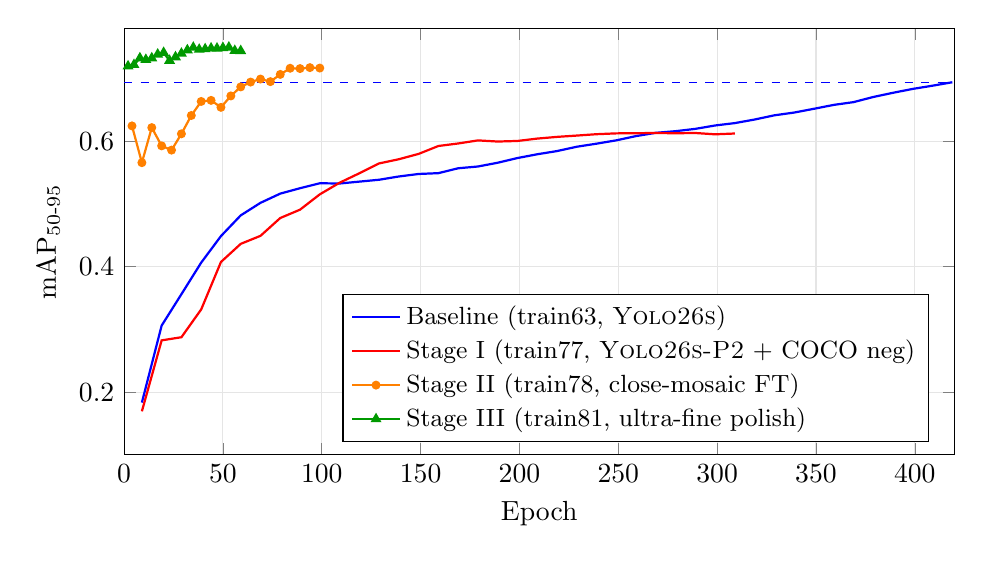
\begin{tikzpicture}
    \begin{axis}[
        width=\textwidth,
        height=7cm,
        xlabel={Epoch},
        ylabel={$\mapfull$},
        xmin=0, xmax=420,
        ymin=0.1, ymax=0.78,
        grid=major,
        grid style={gray!20},
        legend pos=south east,
        legend style={font=\small, cells={anchor=west}},
        every axis plot/.append style={thick},
      ]
      % Baseline (train63)
      \addplot[blue, mark=none] coordinates {
          (9, 0.1834) (19, 0.3061) (29, 0.3561) (39, 0.4064) (49, 0.4487)
          (59, 0.4817) (69, 0.5017) (79, 0.5164) (89, 0.5250) (99, 0.5329)
          (109, 0.5325) (119, 0.5355) (129, 0.5385) (139, 0.5437) (149, 0.5477)
          (159, 0.5490) (169, 0.5568) (179, 0.5596) (189, 0.5656) (199, 0.5731)
          (209, 0.5791) (219, 0.5842) (229, 0.5911) (239, 0.5960) (249, 0.6013)
          (259, 0.6081) (269, 0.6133) (279, 0.6159) (289, 0.6196) (299, 0.6250)
          (309, 0.6288) (319, 0.6345) (329, 0.6412) (339, 0.6456) (349, 0.6516)
          (359, 0.6578) (369, 0.6622) (379, 0.6704) (389, 0.6771) (399, 0.6833)
          (409, 0.6884) (419, 0.6939)
        };
      \addlegendentry{Baseline (train63, \yolobase)}

      % Stage I (train77)
      \addplot[red, mark=none] coordinates {
          (9, 0.1694) (19, 0.2825) (29, 0.2875) (39, 0.3318) (49, 0.4074)
          (59, 0.4363) (69, 0.4491) (79, 0.4775) (89, 0.4908) (99, 0.5152)
          (109, 0.5337) (119, 0.5488) (129, 0.5645) (139, 0.5712) (149, 0.5797)
          (159, 0.5923) (169, 0.5963) (179, 0.6012) (189, 0.5994) (199, 0.6003)
          (209, 0.6041) (219, 0.6068) (229, 0.6089) (239, 0.6111) (249, 0.6124)
          (259, 0.6127) (269, 0.6130) (279, 0.6126) (289, 0.6130) (299, 0.6109)
          (309, 0.6122)
        };
      \addlegendentry{Stage~I (train77, \yolop{} + COCO neg)}

      % Stage II (train78) -- offset by train77 epochs
      \addplot[orange, mark=*, mark size=1.2pt] coordinates {
          (4, 0.6243) (9, 0.5657) (14, 0.6216) (19, 0.5925) (24, 0.5857)
          (29, 0.6117) (34, 0.6409) (39, 0.6633) (44, 0.6650) (49, 0.6539)
          (54, 0.6721) (59, 0.6865) (64, 0.6942) (69, 0.6990) (74, 0.6949)
          (79, 0.7064) (84, 0.7162) (89, 0.7157) (94, 0.7172) (99, 0.7165)
        };
      \addlegendentry{Stage~II (train78, close-mosaic FT)}

      % Stage III (train81)
      \addplot[green!60!black, mark=triangle*, mark size=1.5pt] coordinates {
          (2, 0.7195) (5, 0.7217) (8, 0.7323) (11, 0.7298) (14, 0.7323)
          (17, 0.7383) (20, 0.7410) (23, 0.7284) (26, 0.7340) (29, 0.7397)
          (32, 0.7451) (35, 0.7492) (38, 0.7460) (41, 0.7468) (44, 0.7480)
          (47, 0.7479) (50, 0.7487) (53, 0.7495) (56, 0.7441) (59, 0.7439)
        };
      \addlegendentry{Stage~III (train81, ultra-fine polish)}

      % Horizontal reference line for baseline best
      \addplot[blue, dashed, thin] coordinates {(0, 0.694) (420, 0.694)};

    \end{axis}
  \end{tikzpicture}
  \caption{$\mapfull$ learning curves across all stages.  The dashed
    blue line marks the baseline best ($0.694$).  Stage~II and III are
    plotted on their own epoch axes.  Stage~II shows the dramatic recovery
    once mosaic is disabled.}
  \label{fig:map_curves}
\end{figure}

\subsection{Validation Loss Curves}

\Cref{fig:val_loss} compares the validation box loss between the
baseline and Stage~I, revealing the convergence pattern.

\begin{figure}[H]
  \centering
  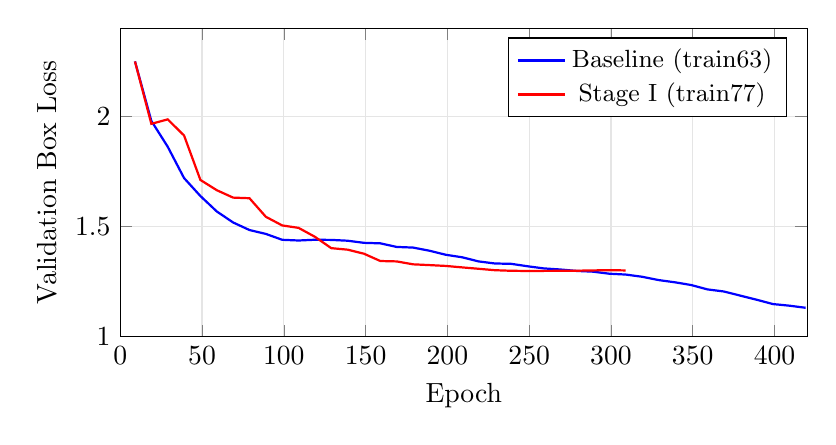
\begin{tikzpicture}
    \begin{axis}[
        width=0.85\textwidth,
        height=5.5cm,
        xlabel={Epoch},
        ylabel={Validation Box Loss},
        xmin=0, xmax=420,
        ymin=1.0, ymax=2.4,
        grid=major,
        grid style={gray!20},
        legend pos=north east,
        legend style={font=\small},
        every axis plot/.append style={thick},
      ]
      \addplot[blue, mark=none] coordinates {
          (9, 2.2495) (19, 1.9797) (29, 1.8625) (39, 1.7202) (49, 1.6386)
          (59, 1.5687) (69, 1.5186) (79, 1.4843) (89, 1.4667) (99, 1.4400)
          (109, 1.4368) (119, 1.4402) (129, 1.4395) (139, 1.4358) (149, 1.4262)
          (159, 1.4239) (169, 1.4076) (179, 1.4047) (189, 1.3905) (199, 1.3721)
          (209, 1.3607) (219, 1.3420) (229, 1.3325) (239, 1.3309) (249, 1.3199)
          (259, 1.3101) (269, 1.3053) (279, 1.2987) (289, 1.2954) (299, 1.2861)
          (309, 1.2823) (319, 1.2723) (329, 1.2574) (339, 1.2472) (349, 1.2348)
          (359, 1.2149) (369, 1.2055) (379, 1.1868) (389, 1.1682) (399, 1.1484)
          (409, 1.1411) (419, 1.1315)
        };
      \addlegendentry{Baseline (train63)}

      \addplot[red, mark=none] coordinates {
          (9, 2.2492) (19, 1.9662) (29, 1.9864) (39, 1.9134) (49, 1.7116)
          (59, 1.6651) (69, 1.6314) (79, 1.6286) (89, 1.5444) (99, 1.5052)
          (109, 1.4941) (119, 1.4536) (129, 1.4021) (139, 1.3952) (149, 1.3768)
          (159, 1.3437) (169, 1.3419) (179, 1.3287) (189, 1.3252) (199, 1.3214)
          (209, 1.3148) (219, 1.3085) (229, 1.3020) (239, 1.2994) (249, 1.2985)
          (259, 1.2989) (269, 1.2992) (279, 1.2997) (289, 1.3011) (299, 1.3021)
          (309, 1.3010)
        };
      \addlegendentry{Stage~I (train77)}

    \end{axis}
  \end{tikzpicture}
  \caption{Validation box loss comparison.  The baseline (train63,
    \yolobase) continues to decrease throughout 420 epochs, while
    Stage~I (train77, \yolop) \emph{stagnates} around epoch~250 and
    begins to \emph{slightly increase}---a sign that the model benefits
    from distribution shift (disabling mosaic) rather than more of the
    same augmented data.}
  \label{fig:val_loss}
\end{figure}

\subsection{Stage-by-Stage Improvement Breakdown}

\begin{figure}[H]
  \centering
  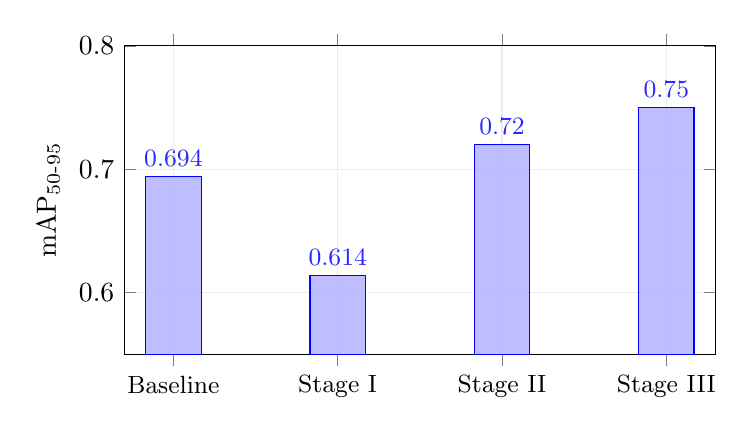
\begin{tikzpicture}
    \begin{axis}[
        ybar,
        width=0.75\textwidth,
        height=5.5cm,
        bar width=20pt,
        ylabel={$\mapfull$},
        symbolic x coords={Baseline, {Stage I}, {Stage II}, {Stage III}},
        xtick=data,
        xticklabel style={font=\small},
        ymin=0.55, ymax=0.80,
        nodes near coords,
        nodes near coords style={font=\small\bfseries, above},
        every node near coord/.append style={/pgf/number format/.cd, fixed, precision=3},
        grid=major,
        grid style={gray!15},
        every axis plot/.append style={fill opacity=0.85},
      ]
      \addplot coordinates {(Baseline, 0.694) ({Stage I}, 0.614) ({Stage II}, 0.720) ({Stage III}, 0.750)};
    \end{axis}
  \end{tikzpicture}
  \caption{$\mapfull$ progression across training stages.  The initial
    drop from Baseline to Stage~I is due to the harder training
    distribution (COCO negatives + mosaic-only training).  Stages II and
    III progressively recover and exceed the baseline.}
  \label{fig:bar}
\end{figure}

\subsection{Precision--Recall Curves}

\Cref{fig:pr_curves} shows the precision--recall curves for the
baseline and the final model, generated by Ultralytics.

\begin{figure}[H]
  \centering
  \begin{subfigure}[t]{0.48\textwidth}
    \centering
    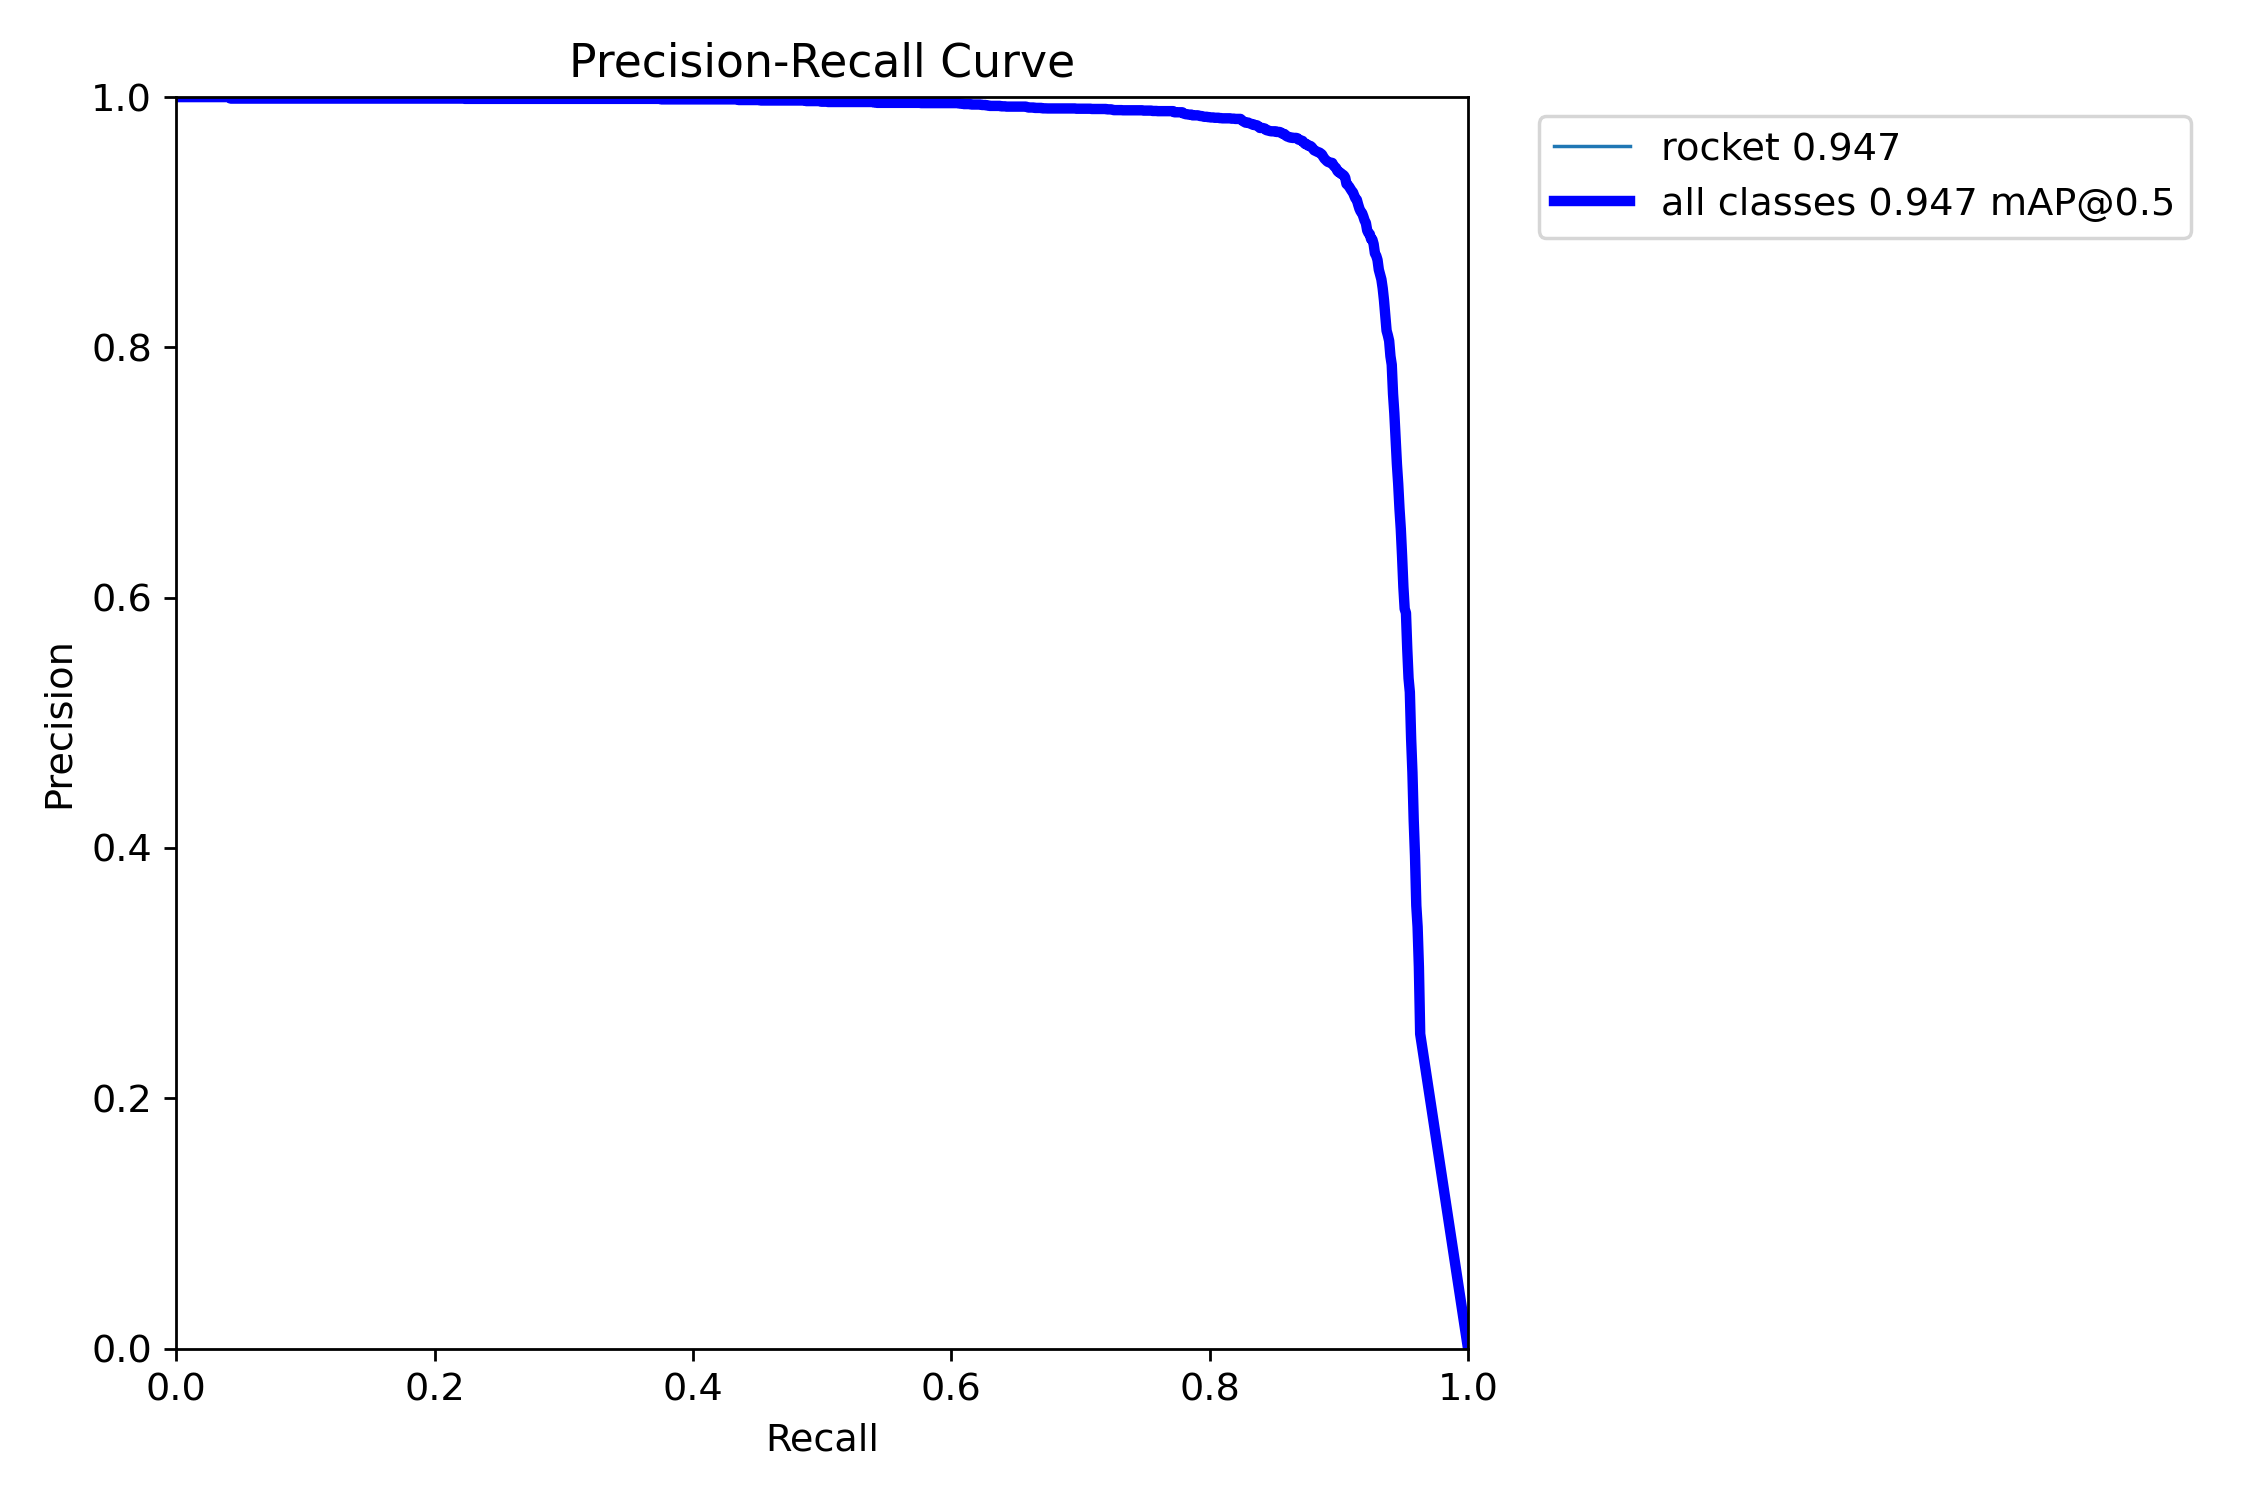
\includegraphics[width=\textwidth]{pr_train63.png}
    \caption{Baseline (train63): $\mapfifty = 0.948$}
  \end{subfigure}
  \hfill
  \begin{subfigure}[t]{0.48\textwidth}
    \centering
    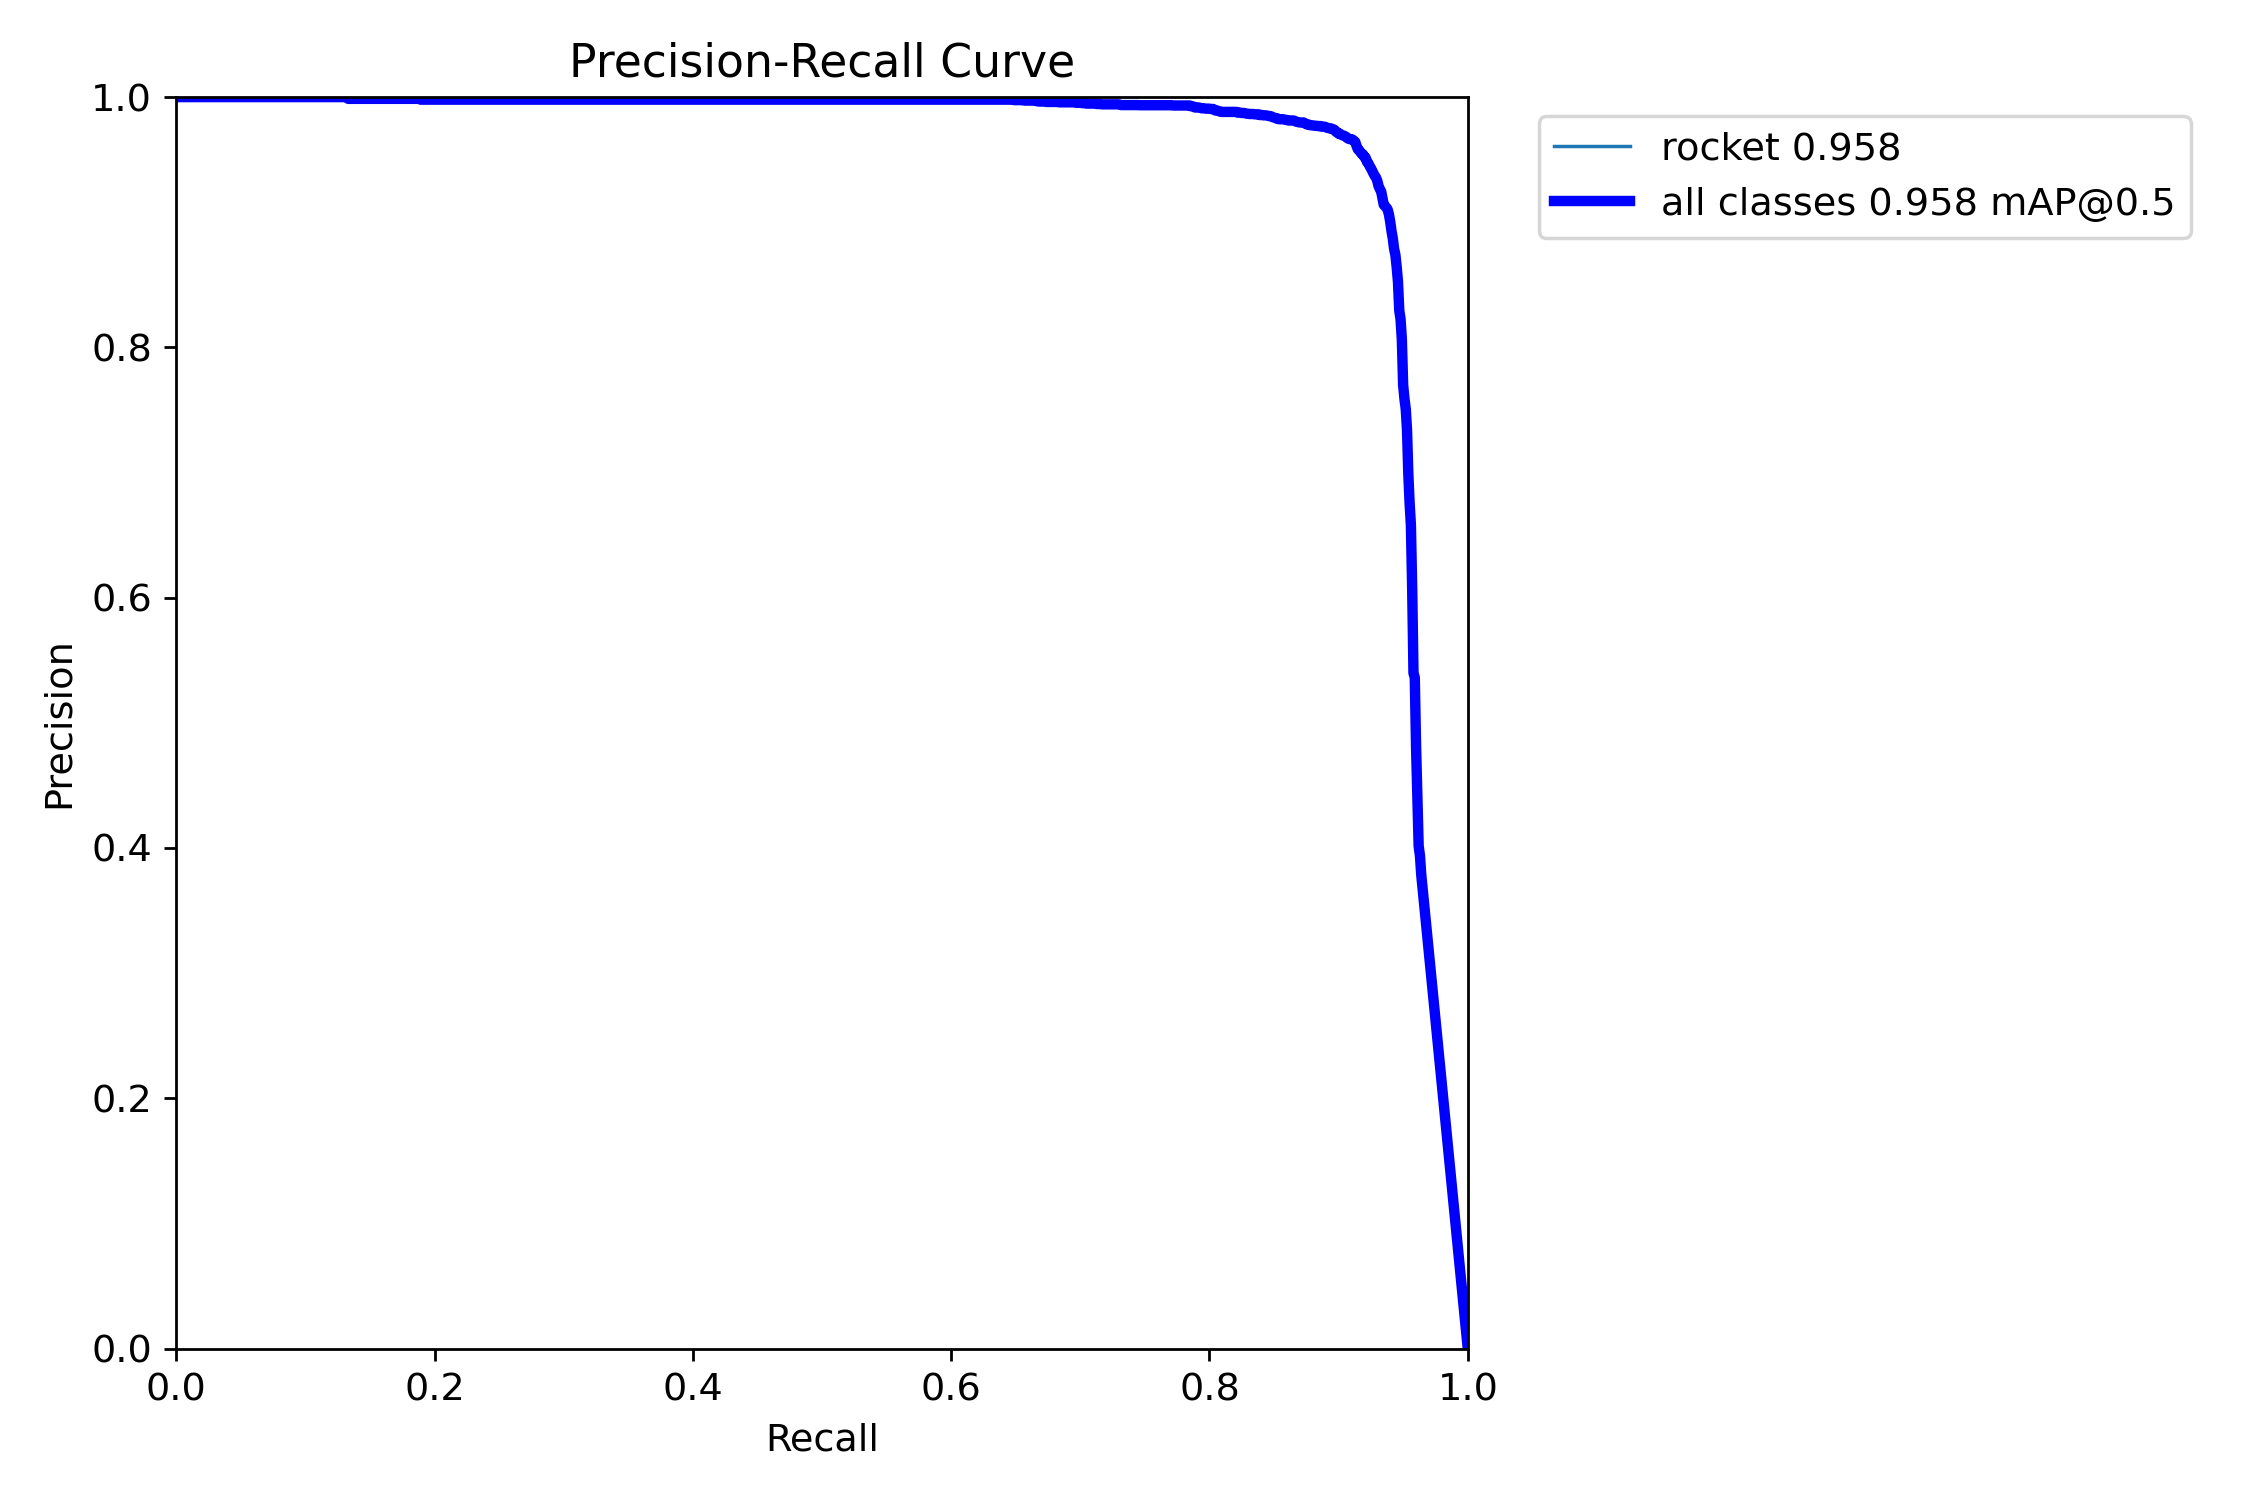
\includegraphics[width=\textwidth]{pr_train81.png}
    \caption{Final model (train81): $\mapfifty = 0.958$}
  \end{subfigure}
  \caption{Precision--Recall curves for the baseline and final model.
    The final model achieves both higher precision and higher recall.}
  \label{fig:pr_curves}
\end{figure}

\subsection{Confusion Matrices}

\Cref{fig:cm} presents the normalised confusion matrices, showing the
reduction in false negatives and false positives.

\begin{figure}[H]
  \centering
  \begin{subfigure}[t]{0.48\textwidth}
    \centering
    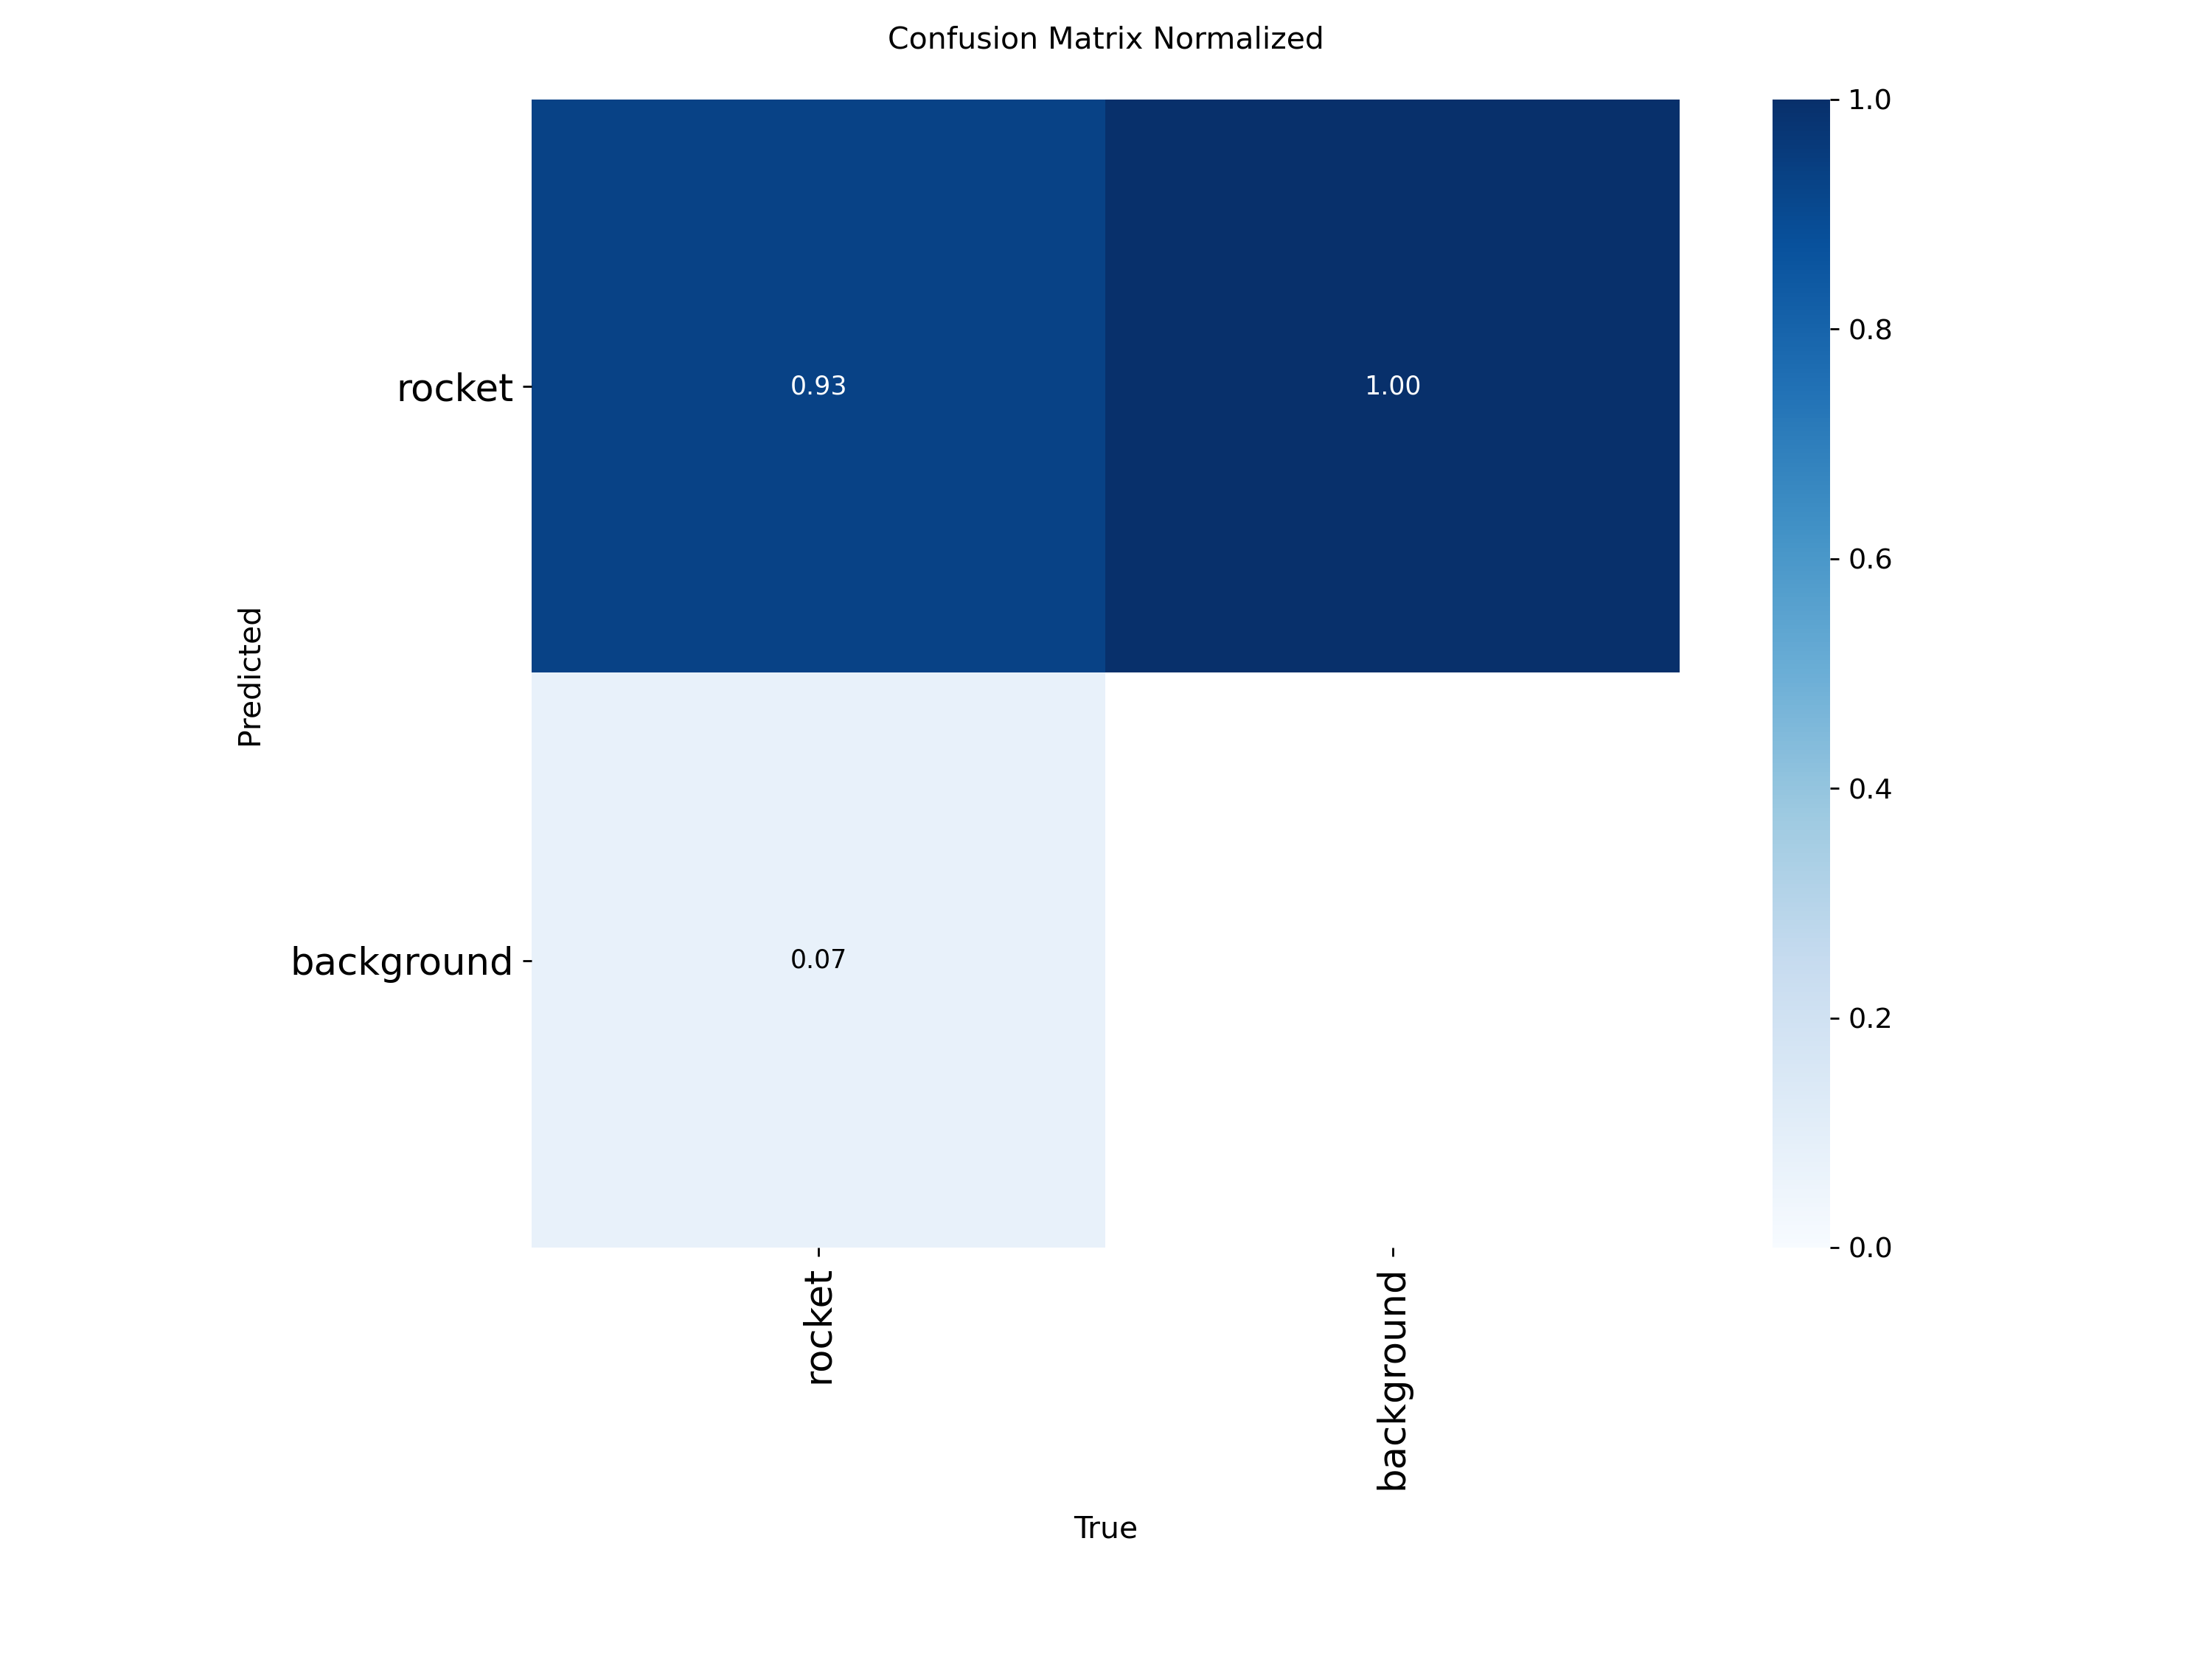
\includegraphics[width=\textwidth]{cm_train63.png}
    \caption{Baseline (train63)}
  \end{subfigure}
  \hfill
  \begin{subfigure}[t]{0.48\textwidth}
    \centering
    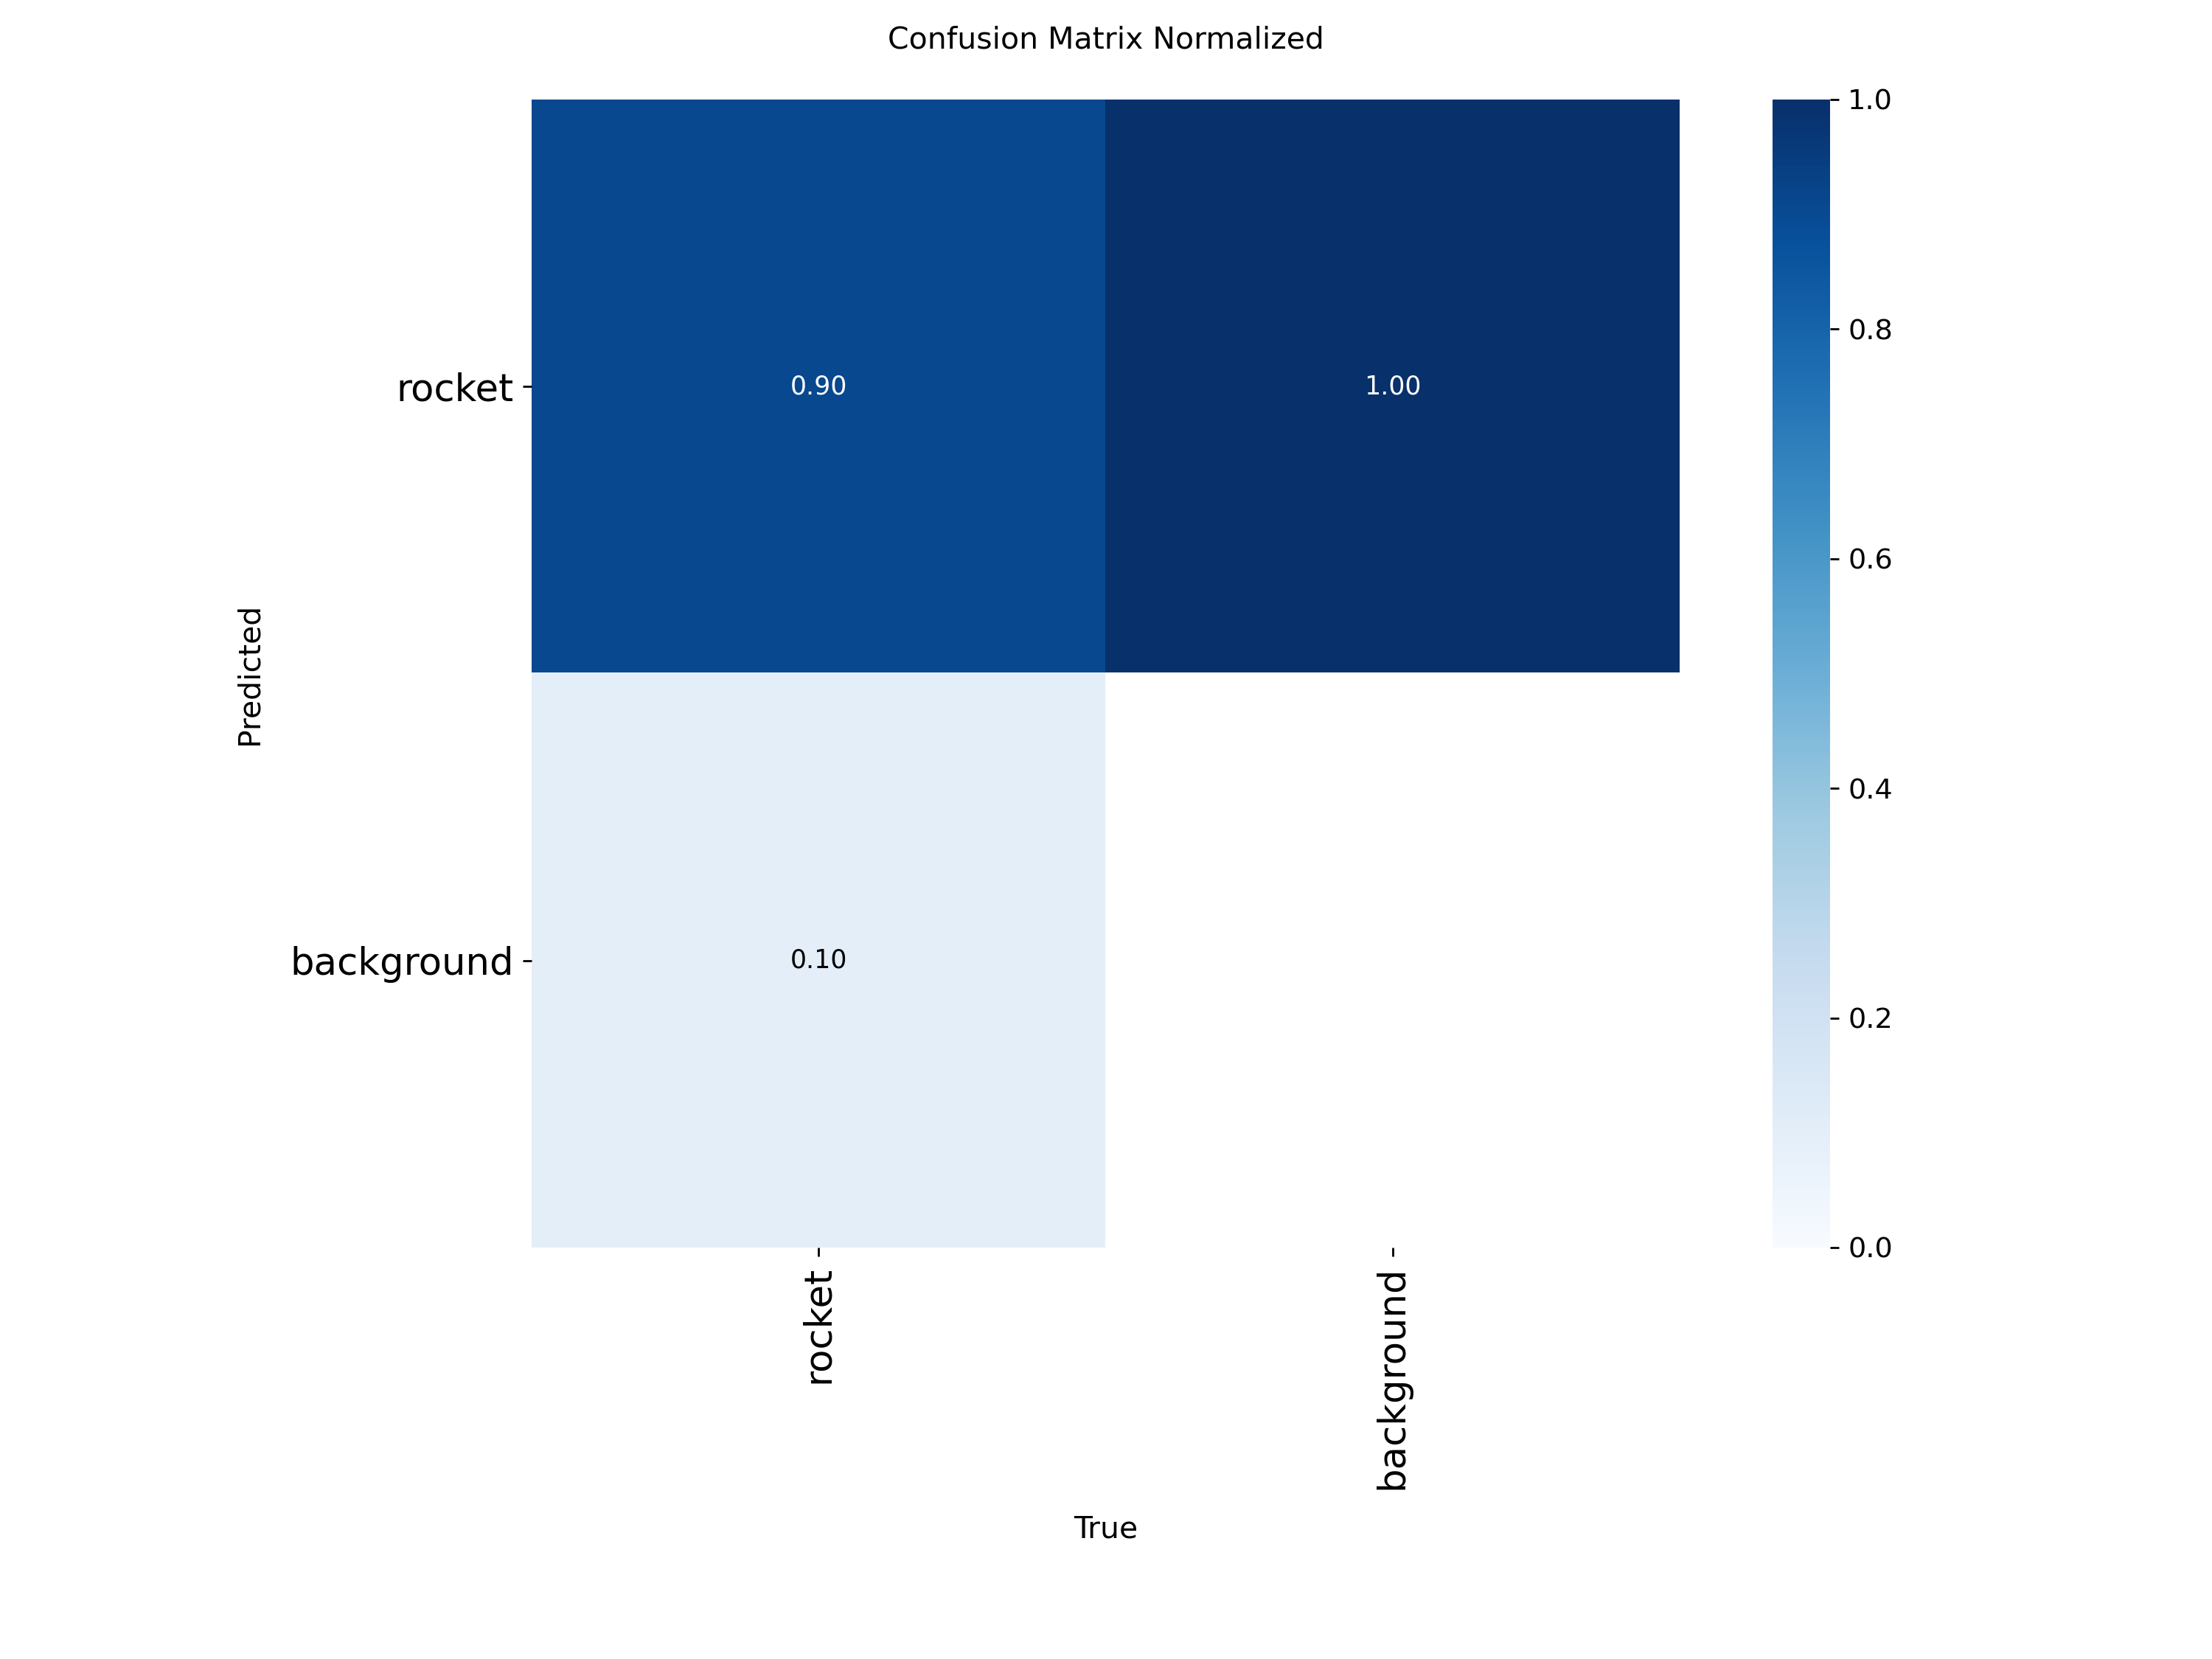
\includegraphics[width=\textwidth]{cm_train81.png}
    \caption{Final model (train81)}
  \end{subfigure}
  \caption{Normalised confusion matrices.  The final model shows
    improved true-positive rate and reduced background confusion.}
  \label{fig:cm}
\end{figure}

\subsection{Qualitative Results}

\Cref{fig:qualitative} provides a visual comparison of detection
quality on validation images.

\begin{figure}[H]
  \centering
  \begin{subfigure}[t]{0.48\textwidth}
    \centering
    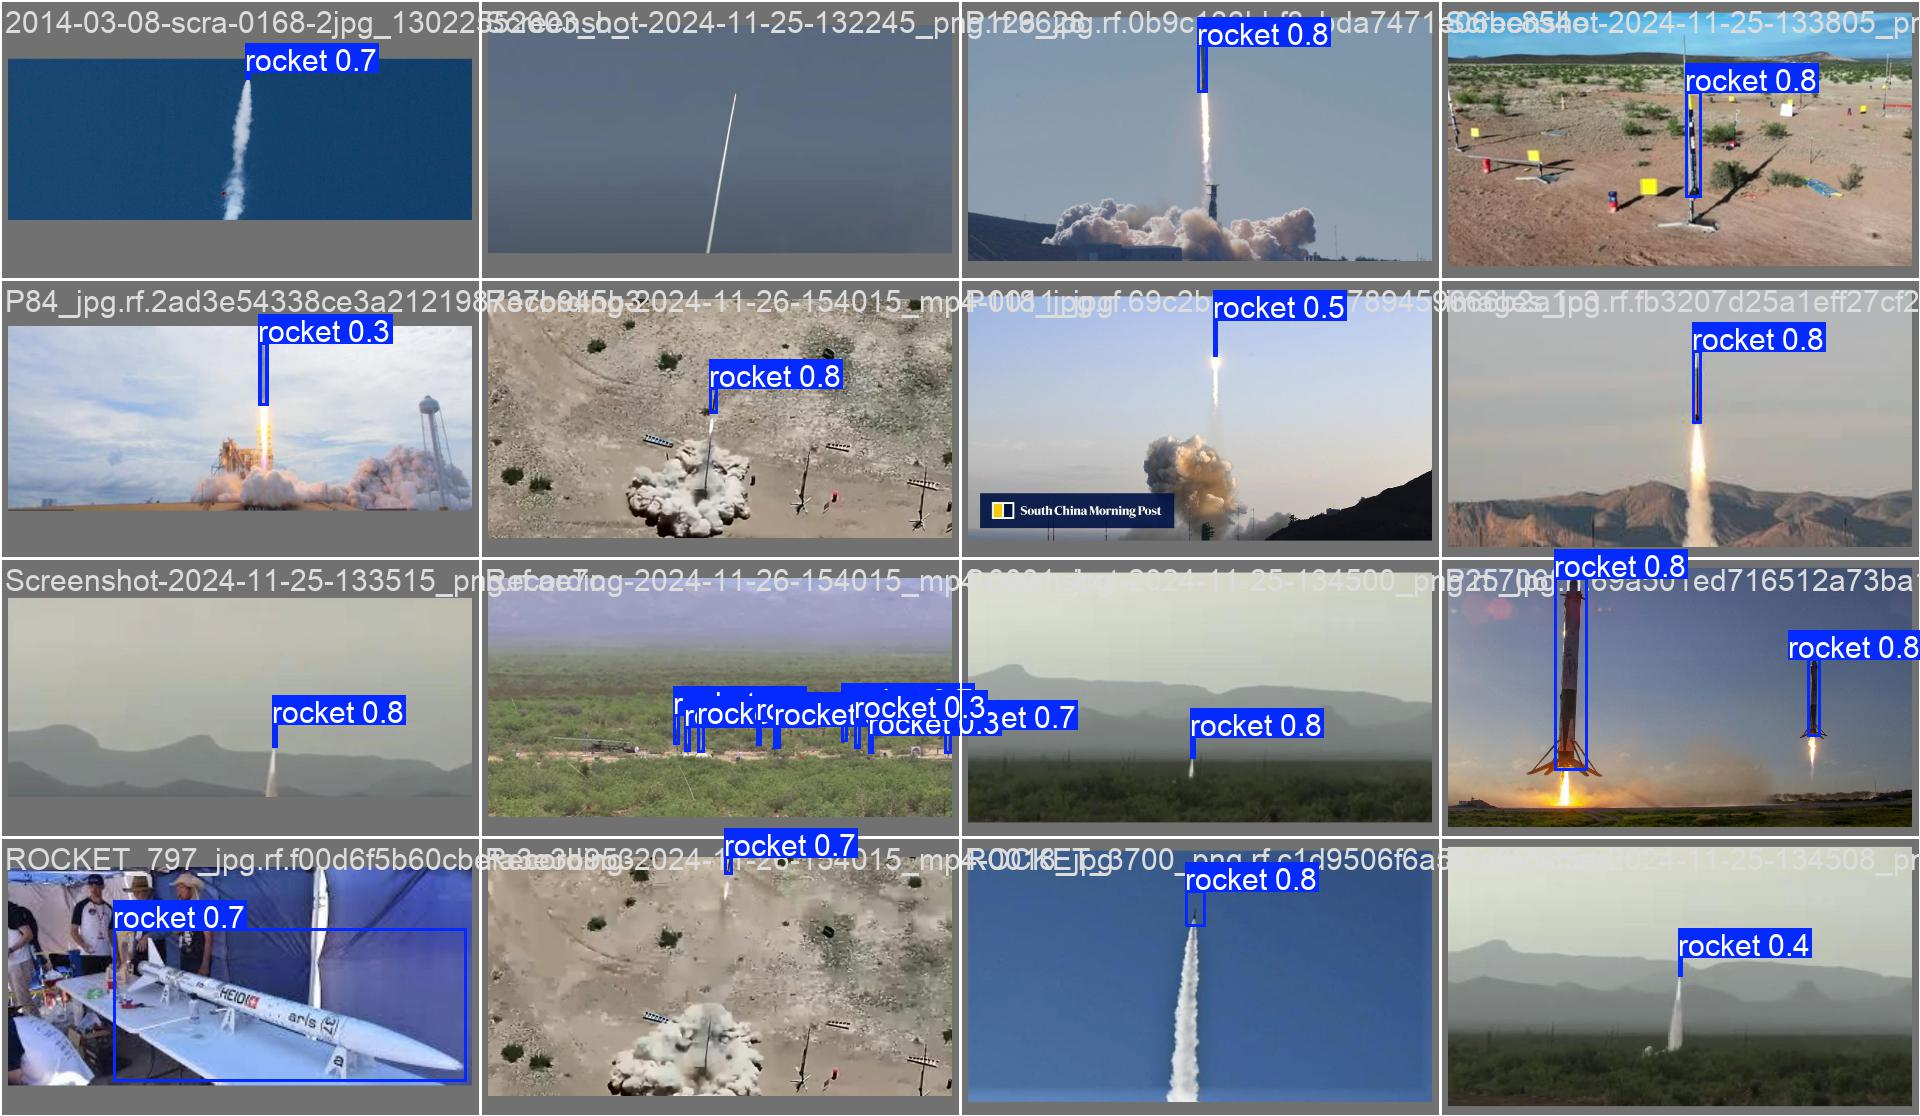
\includegraphics[width=\textwidth]{val_pred_train63.jpg}
    \caption{Baseline predictions (train63)}
  \end{subfigure}
  \hfill
  \begin{subfigure}[t]{0.48\textwidth}
    \centering
    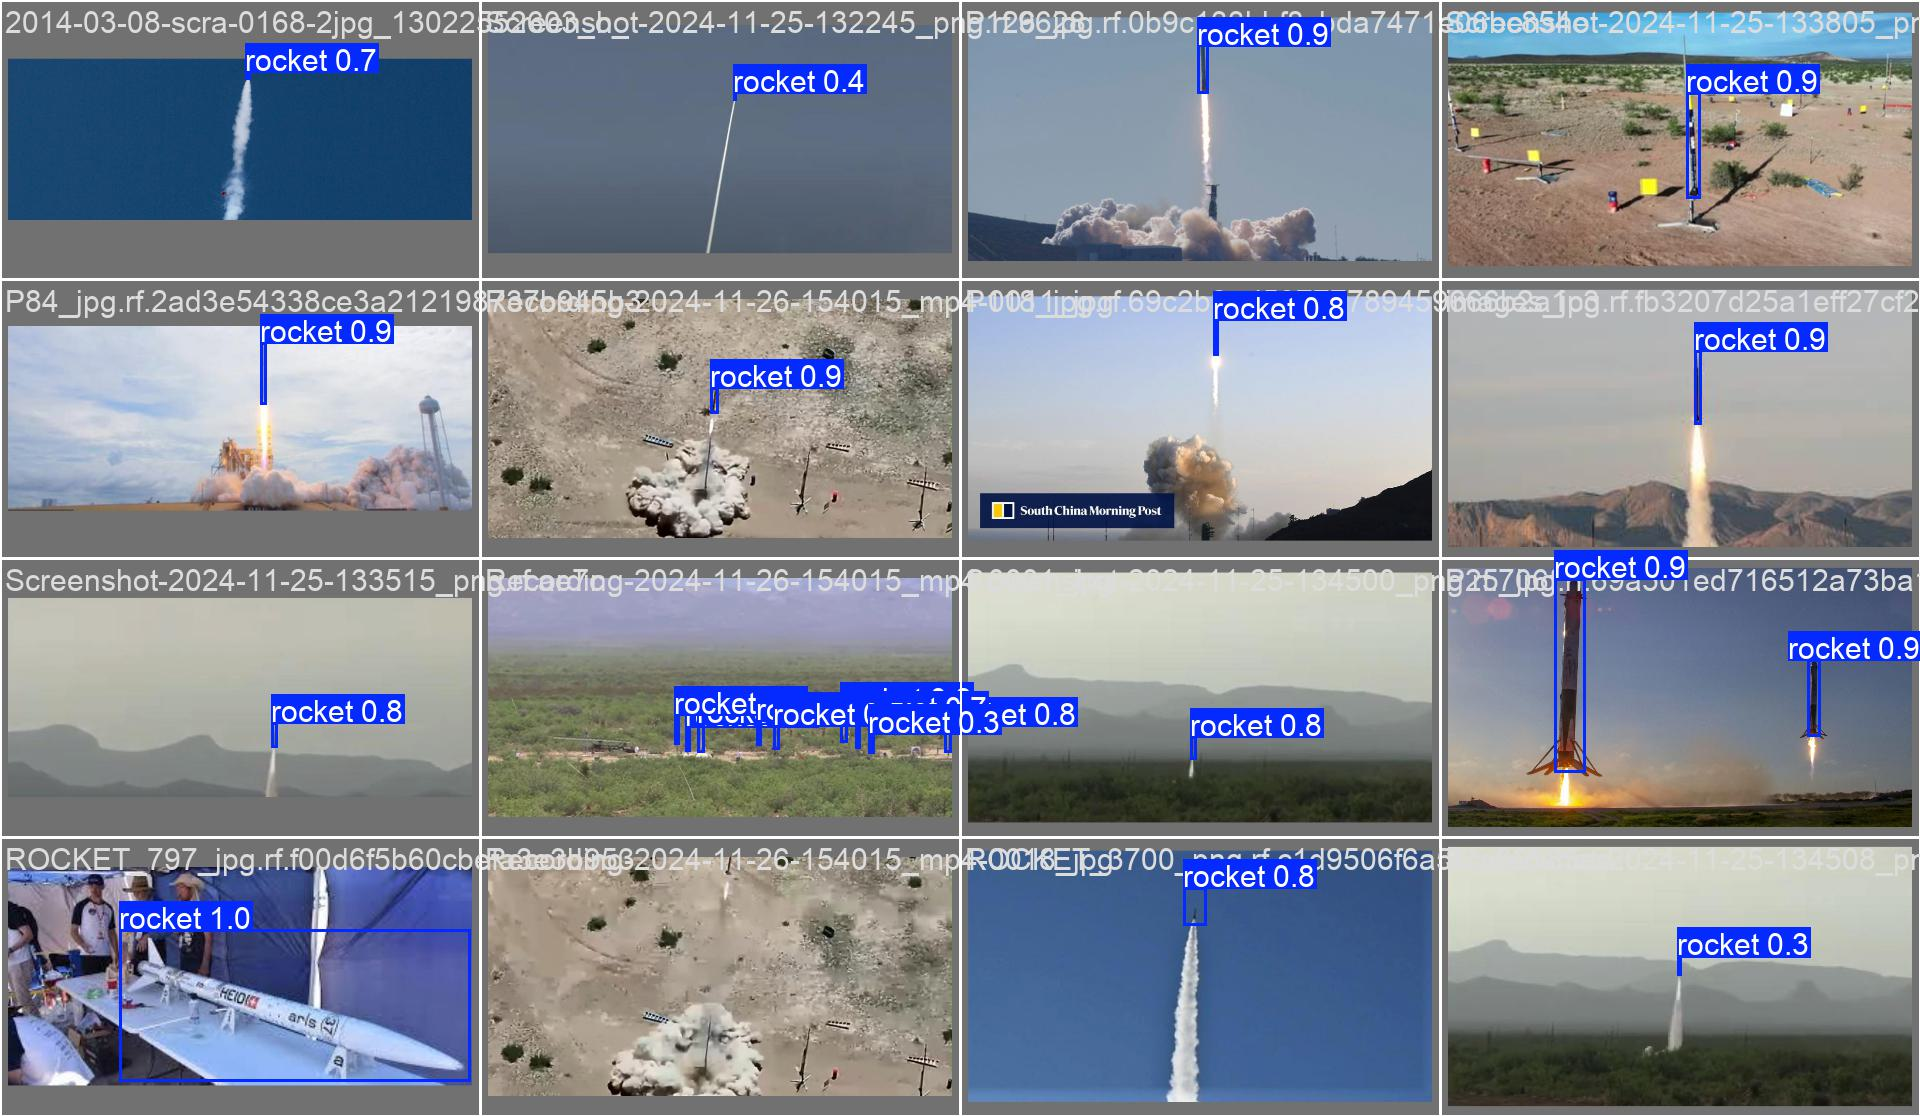
\includegraphics[width=\textwidth]{val_pred_train81.jpg}
    \caption{Final model predictions (train81)}
  \end{subfigure}
  \caption{Validation batch predictions.  The final model produces
    tighter bounding boxes and higher confidence scores, particularly on
    small targets.}
  \label{fig:qualitative}
\end{figure}

% ═══════════════════════════════════════════════════════════════════
\section{Analysis and Discussion}
\label{sec:discussion}

\subsection{Why Did Stage~I Degrade Performance?}

The $\mapfull$ drop from $0.694$ (baseline) to $0.614$ (Stage~I) is
attributable to \textbf{three compounding factors}:

\begin{enumerate}[leftmargin=*]
  \item \textbf{COCO negative dilution}: Adding 4{,}000 background
        images (25\% of training data) forces the model to learn a
        harder decision boundary, trading recall for
        false-positive suppression.  While beneficial for deployment
        (fewer false alarms), this manifests as lower
        $\mapfull$ on the validation set that contains no COCO images.

  \item \textbf{Mosaic starvation}: Mosaic augmentation~\cite{bochkovskiy2020yolov4}
        composites four images into one,
        reducing each to $\frac{1}{4}$ resolution.  For our
        already-small rockets, this pushes targets below the
        detection threshold.  The intended remedy---disabling mosaic
        in the final epochs (\texttt{close\_mosaic})---was
        \emph{never activated} because early stopping triggered first.

  \item \textbf{Architectural cold start}: The P2 head introduces new
        layers initialised from transferred weights that only
        partially match.  These require extended training to specialise
        for the target domain, particularly at the finest scale.
\end{enumerate}

\subsection{The Close-Mosaic Timing Problem}
\label{sec:close_mosaic}

The interaction between \texttt{close\_mosaic} and \texttt{patience} (early
stopping) is a subtle but critical failure mode:

\[
  \text{mosaic\_off\_epoch} = \text{total\_epochs} - \text{close\_mosaic}
  = 600 - 250 = 350
\]

But early stopping triggered at epoch~317 ($<350$), so the transition never
occurred. The solution is to decouple the two by performing close-mosaic
fine-tuning as a \emph{separate training stage} with mosaic explicitly set
to~$0$, which is precisely what Stage~II achieves.

\paragraph{Design recommendation.}  For long training runs with large \texttt{close\_mosaic} windows, either
(a)~set $\text{patience} > \text{epochs} - \text{close\_mosaic\_epoch}$, or
(b)~implement close-mosaic as a separate fine-tuning stage.

\subsection{Effect of COCO Negative Count}

We experimented with two levels of COCO negative injection:

\begin{table}[h]
  \centering
  \caption{Impact of COCO negative sample count.}
  \label{tab:coco_count}
  \begin{tabular}{@{}lccc@{}}
    \toprule
    \textbf{Run}       & \textbf{COCO Negatives} & \textbf{\% of Training Set} & $\mathbf{\mapfull}$ \\
    \midrule
    train63 (baseline) & 0                       & 0\%                         & 0.694               \\
    train76            & 1{,}000                 & 7.8\%                       & 0.652               \\
    train77            & 4{,}000                 & 25.3\%                      & 0.614               \\
    \bottomrule
  \end{tabular}
\end{table}

More negatives produce a harder training problem (lower $\mapfull$) but are
expected to improve \emph{deployment} performance by suppressing false
positives on unseen backgrounds. The 25\% ratio was chosen as a compromise:
enough to provide meaningful false-positive supervision without overwhelming
the positive examples.

\subsection{Diminishing Returns in Stage~III}

Stage~III contributed a $+4.2\%$ improvement to $\mapfull$, compared to
Stage~II's $+17.3\%$. This is expected: as the learning rate decreases
($0.0003$ vs.\ $0.002$), the model makes increasingly small parameter updates.
The $\mapfull$ curve in \Cref{fig:map_curves} shows the Stage~III plateau
beginning around epoch~35, suggesting the model has effectively converged.

\subsection{Optimizer Selection Pitfall}

The failed train79 run highlights an important implementation detail in
Ultralytics: when \texttt{optimizer=``auto''} is set, the framework may
internally select AdamW and apply its own learning-rate scaling heuristics,
effectively \emph{overriding} the user-specified $\text{lr}_0$. For fine-tuning
where precise learning rate control is essential, \textbf{always specify the
  optimizer explicitly}.

% ═══════════════════════════════════════════════════════════════════
\section{Conclusion}
\label{sec:conclusion}

We have presented a systematic, multi-stage training pipeline for small rocket
detection that progresses from a vanilla \yolobase{} baseline ($\mapfull =
  0.694$) to a final \yolop{} model achieving $\mapfull = 0.750$ and $\mapfifty =
  0.958$. The key insights are:

\begin{enumerate}[leftmargin=*]
  \item \textbf{Architecture and data changes must be coupled with
          training strategy.}  The P2 head and COCO negatives initially
        degraded performance; only through staged fine-tuning was
        their potential unlocked.

  \item \textbf{Close-mosaic is critical for small objects.}
        Training exclusively on mosaic-augmented images limits
        small-target localisation.  Disabling mosaic via a dedicated
        fine-tuning stage produced the largest single improvement
        ($+17.3\%$ $\mapfull$).

  \item \textbf{Progressive augmentation reduction} follows the
        principle of curriculum learning: heavy augmentation for
        feature diversity, then minimal augmentation for precision.

  \item \textbf{Deployment considerations.}  The final model runs
        at $960{\times}544$ resolution with ${\sim}9.8$M parameters,
        suitable for real-time inference on GPU-equipped edge devices.
\end{enumerate}

\noindent The complete training pipeline---from COCO download to
final polishing---is implemented in four Python scripts, enabling
full reproducibility.

% ═══════════════════════════════════════════════════════════════════
\appendix
\section{Hardware Configuration}
\label{app:hardware}

\begin{table}[h]
  \centering
  \caption{Training infrastructure.}
  \label{tab:hardware}
  \begin{tabular}{@{}ll@{}}
    \toprule
    \textbf{Component} & \textbf{Specification}                         \\
    \midrule
    GPU                & $4{\times}$ NVIDIA H100 PCIe, 81\,GB HBM3 each \\
    Training mode      & Distributed Data Parallel (DDP), NCCL backend  \\
    Precision          & Mixed (AMP, FP16/FP32)                         \\
    Batch size         & 192 total (48 per GPU)                         \\
    Disk cache         & Enabled (\texttt{cache=`disk'})                \\
    Workers            & 8 per process                                  \\
    \bottomrule
  \end{tabular}
\end{table}

\section{Complete Hyperparameter Table}
\label{app:hyperparams}

\begin{table}[H]
  \centering
  \caption{Full training hyperparameters across all stages.}
  \label{tab:full_hyper}
  \small
  \begin{tabular}{@{}lcccc@{}}
    \toprule
    \textbf{Hyperparameter}  & \textbf{Baseline} & \textbf{Stage~I} & \textbf{Stage~II} & \textbf{Stage~III} \\
                             & (train63)         & (train77)        & (train78)         & (train81)          \\
    \midrule
    Model                    & yolo26s.pt        & yolo26s-p2.yaml  & (from train77)    & (from train78)     \\
    GPUs                     & 1                 & 4                & 4                 & 4                  \\
    Batch                    & 64                & 192              & 192               & 192                \\
    Image size               & $544{\times}960$  & 960              & 960               & 960                \\
    Epochs                   & 420               & 600              & 100               & 60                 \\
    Patience                 & 30                & 50               & 40                & 25                 \\
    Optimizer                & auto              & auto             & auto              & SGD                \\
    $\text{lr}_0$            & 0.01              & 0.01             & 0.002             & 0.0003             \\
    $\text{lrf}$             & 0.01              & 0.02             & 0.05              & 0.2                \\
    Schedule                 & linear            & linear           & cosine            & cosine             \\
    Warmup (ep)              & 3                 & 3                & 5                 & 2                  \\
    multi\_scale             & True              & True             & True              & False              \\
    COCO neg.                & 0                 & 4{,}000          & 4{,}000           & 4{,}000            \\
    \midrule
    \textbf{Best $\mapfull$} & \textbf{0.694}    & \textbf{0.614}   & \textbf{0.720}    & \textbf{0.750}     \\
    \bottomrule
  \end{tabular}
\end{table}

\section{Training Results Plots (Ultralytics)}
\label{app:results_plots}

\Cref{fig:ultralytics_plots} shows the built-in Ultralytics training
results plots for each stage.

\begin{figure}[H]
  \centering
  \begin{subfigure}[t]{0.48\textwidth}
    \centering
    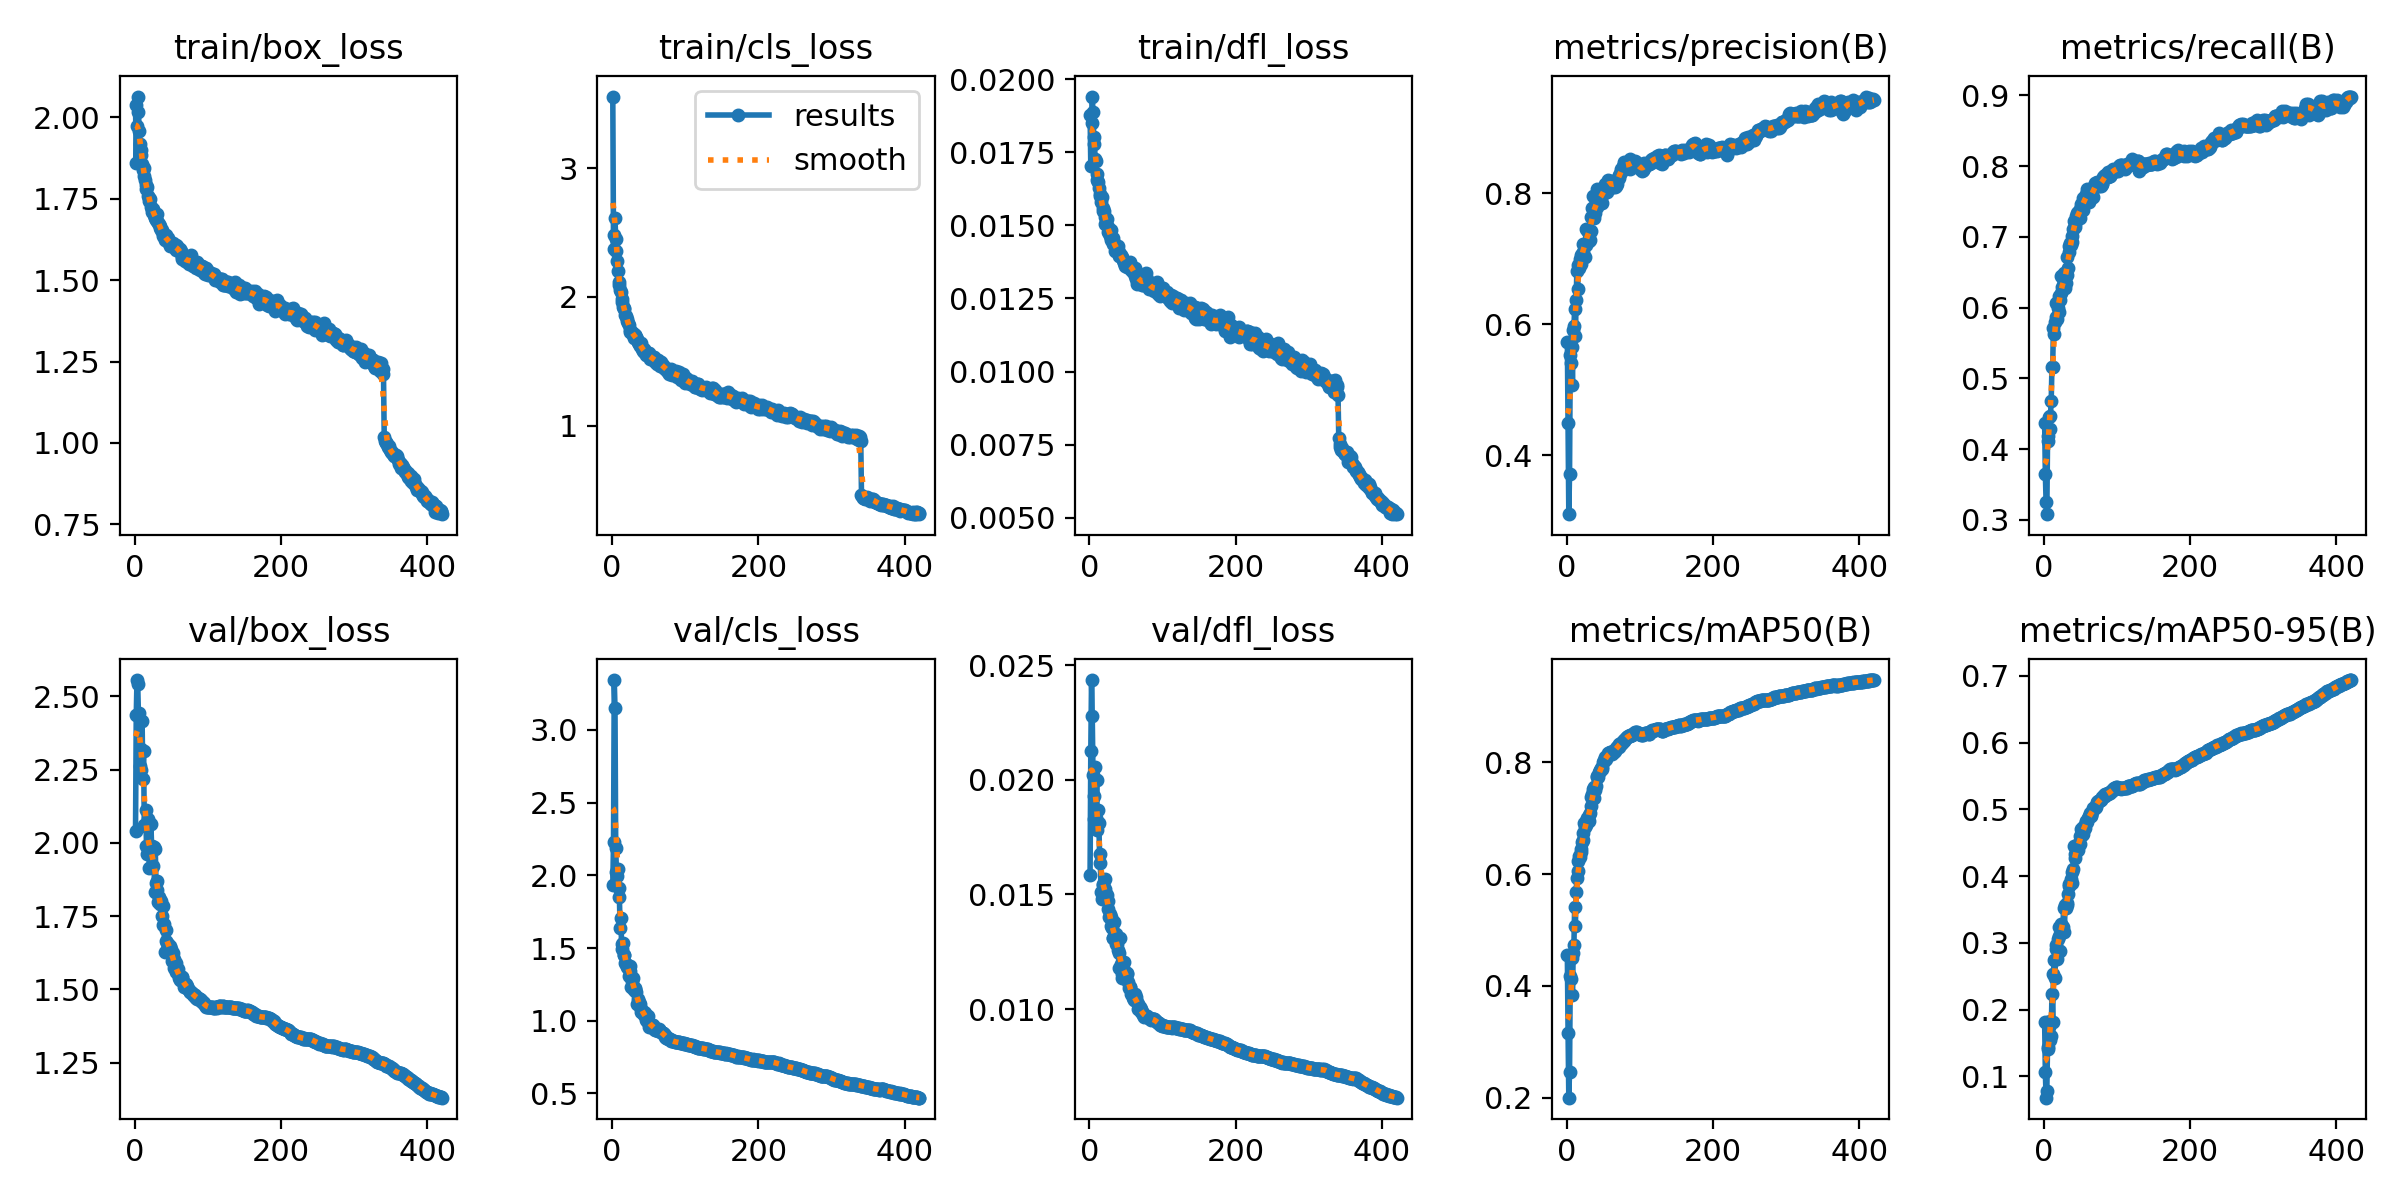
\includegraphics[width=\textwidth]{results_train63.png}
    \caption{Baseline (train63, 420 epochs)}
  \end{subfigure}
  \hfill
  \begin{subfigure}[t]{0.48\textwidth}
    \centering
    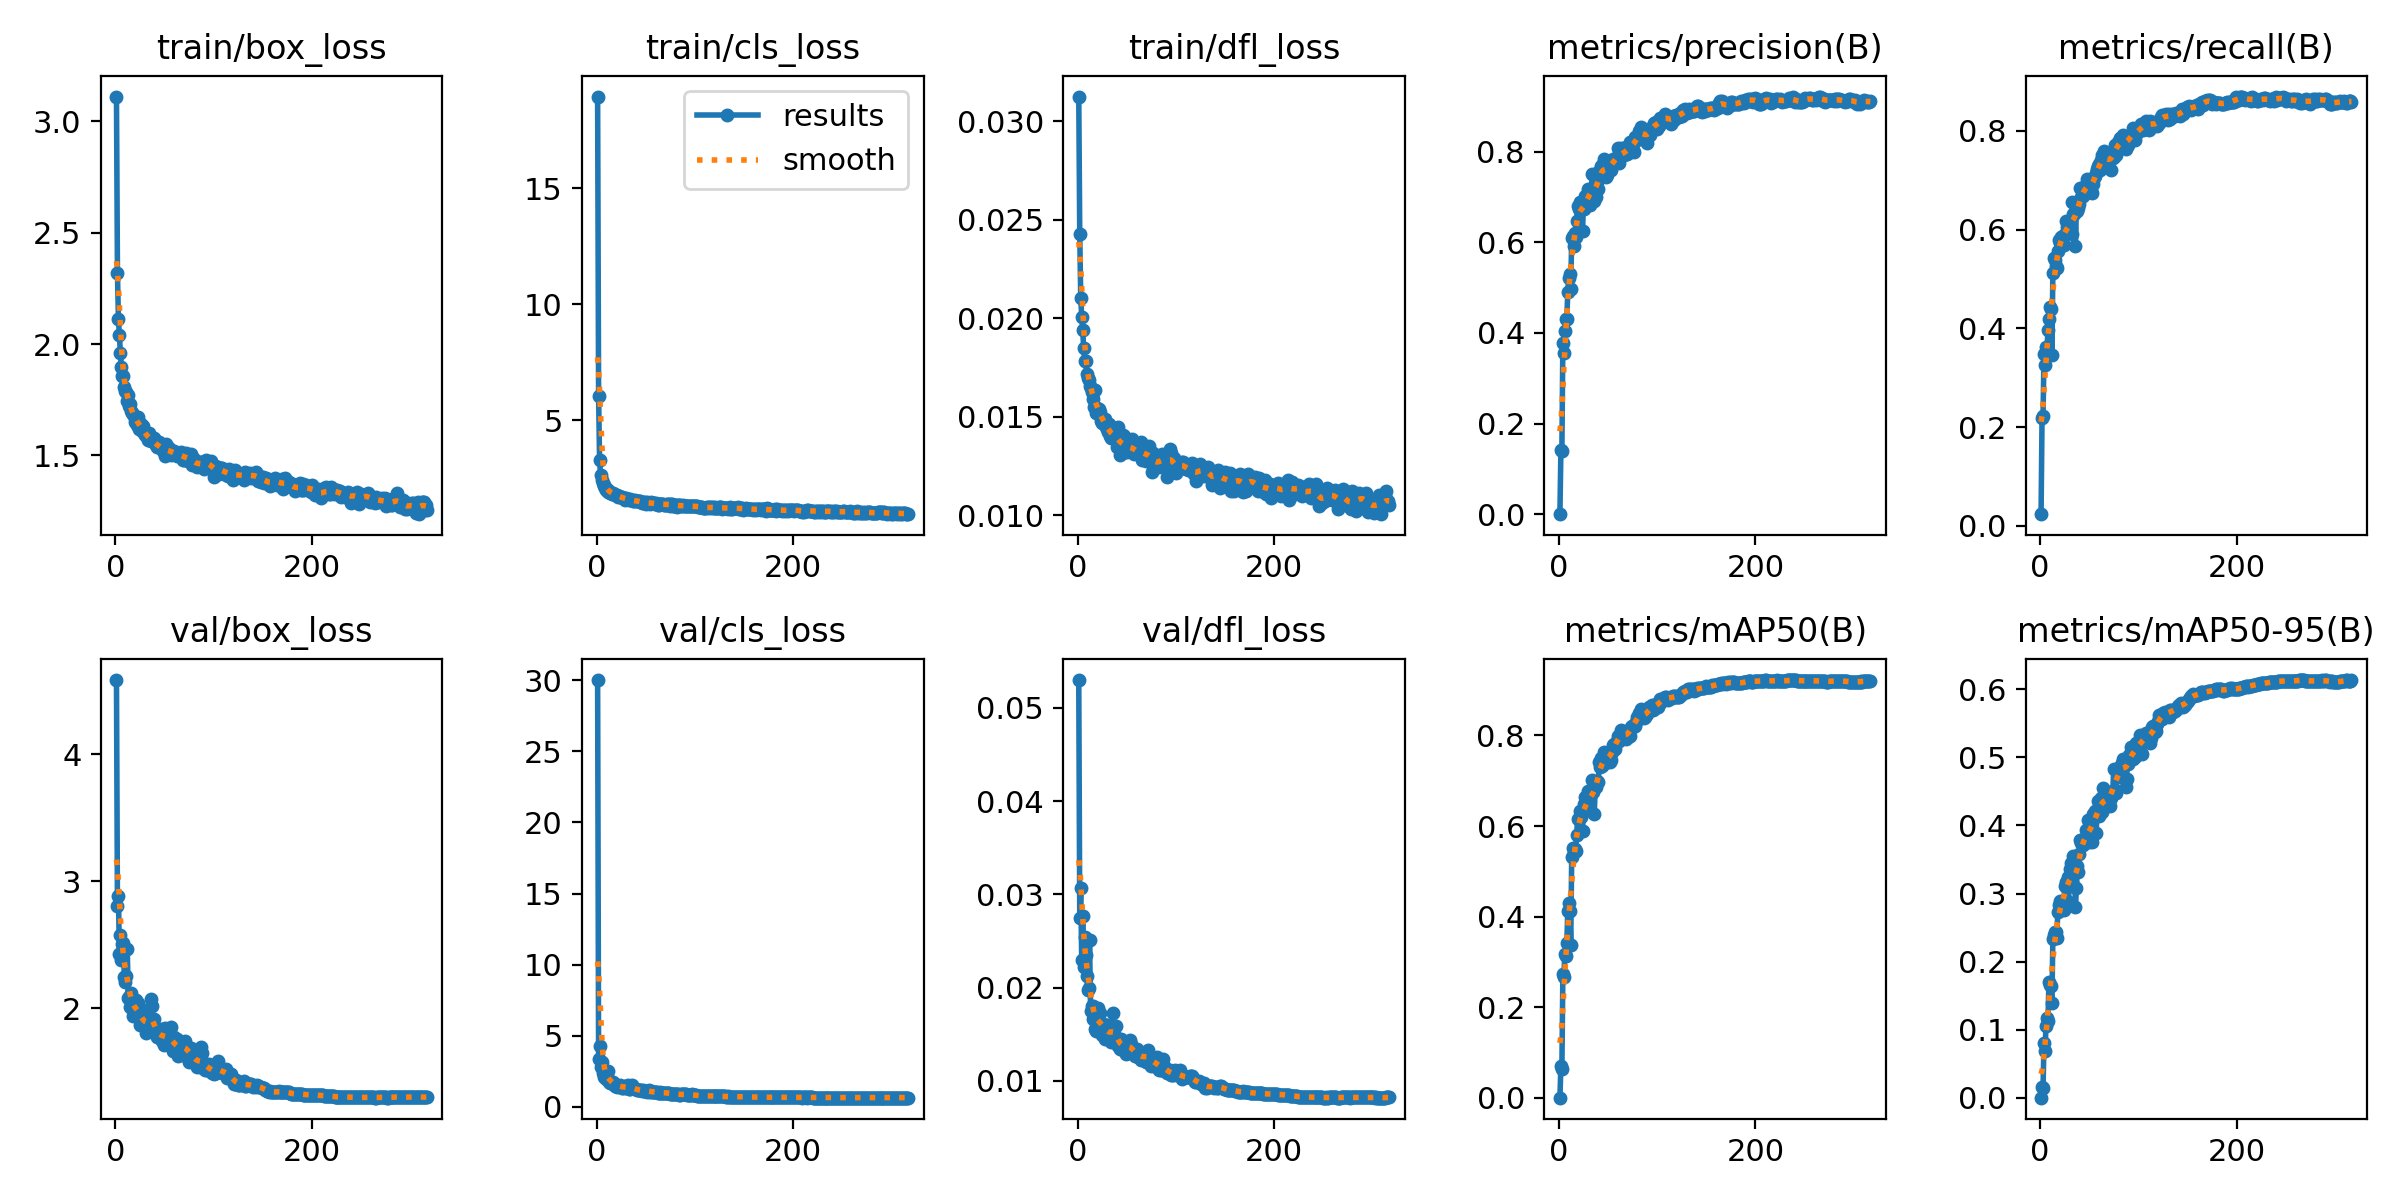
\includegraphics[width=\textwidth]{results_train77.png}
    \caption{Stage~I (train77, 317 epochs)}
  \end{subfigure}

  \vspace{0.5cm}

  \begin{subfigure}[t]{0.48\textwidth}
    \centering
    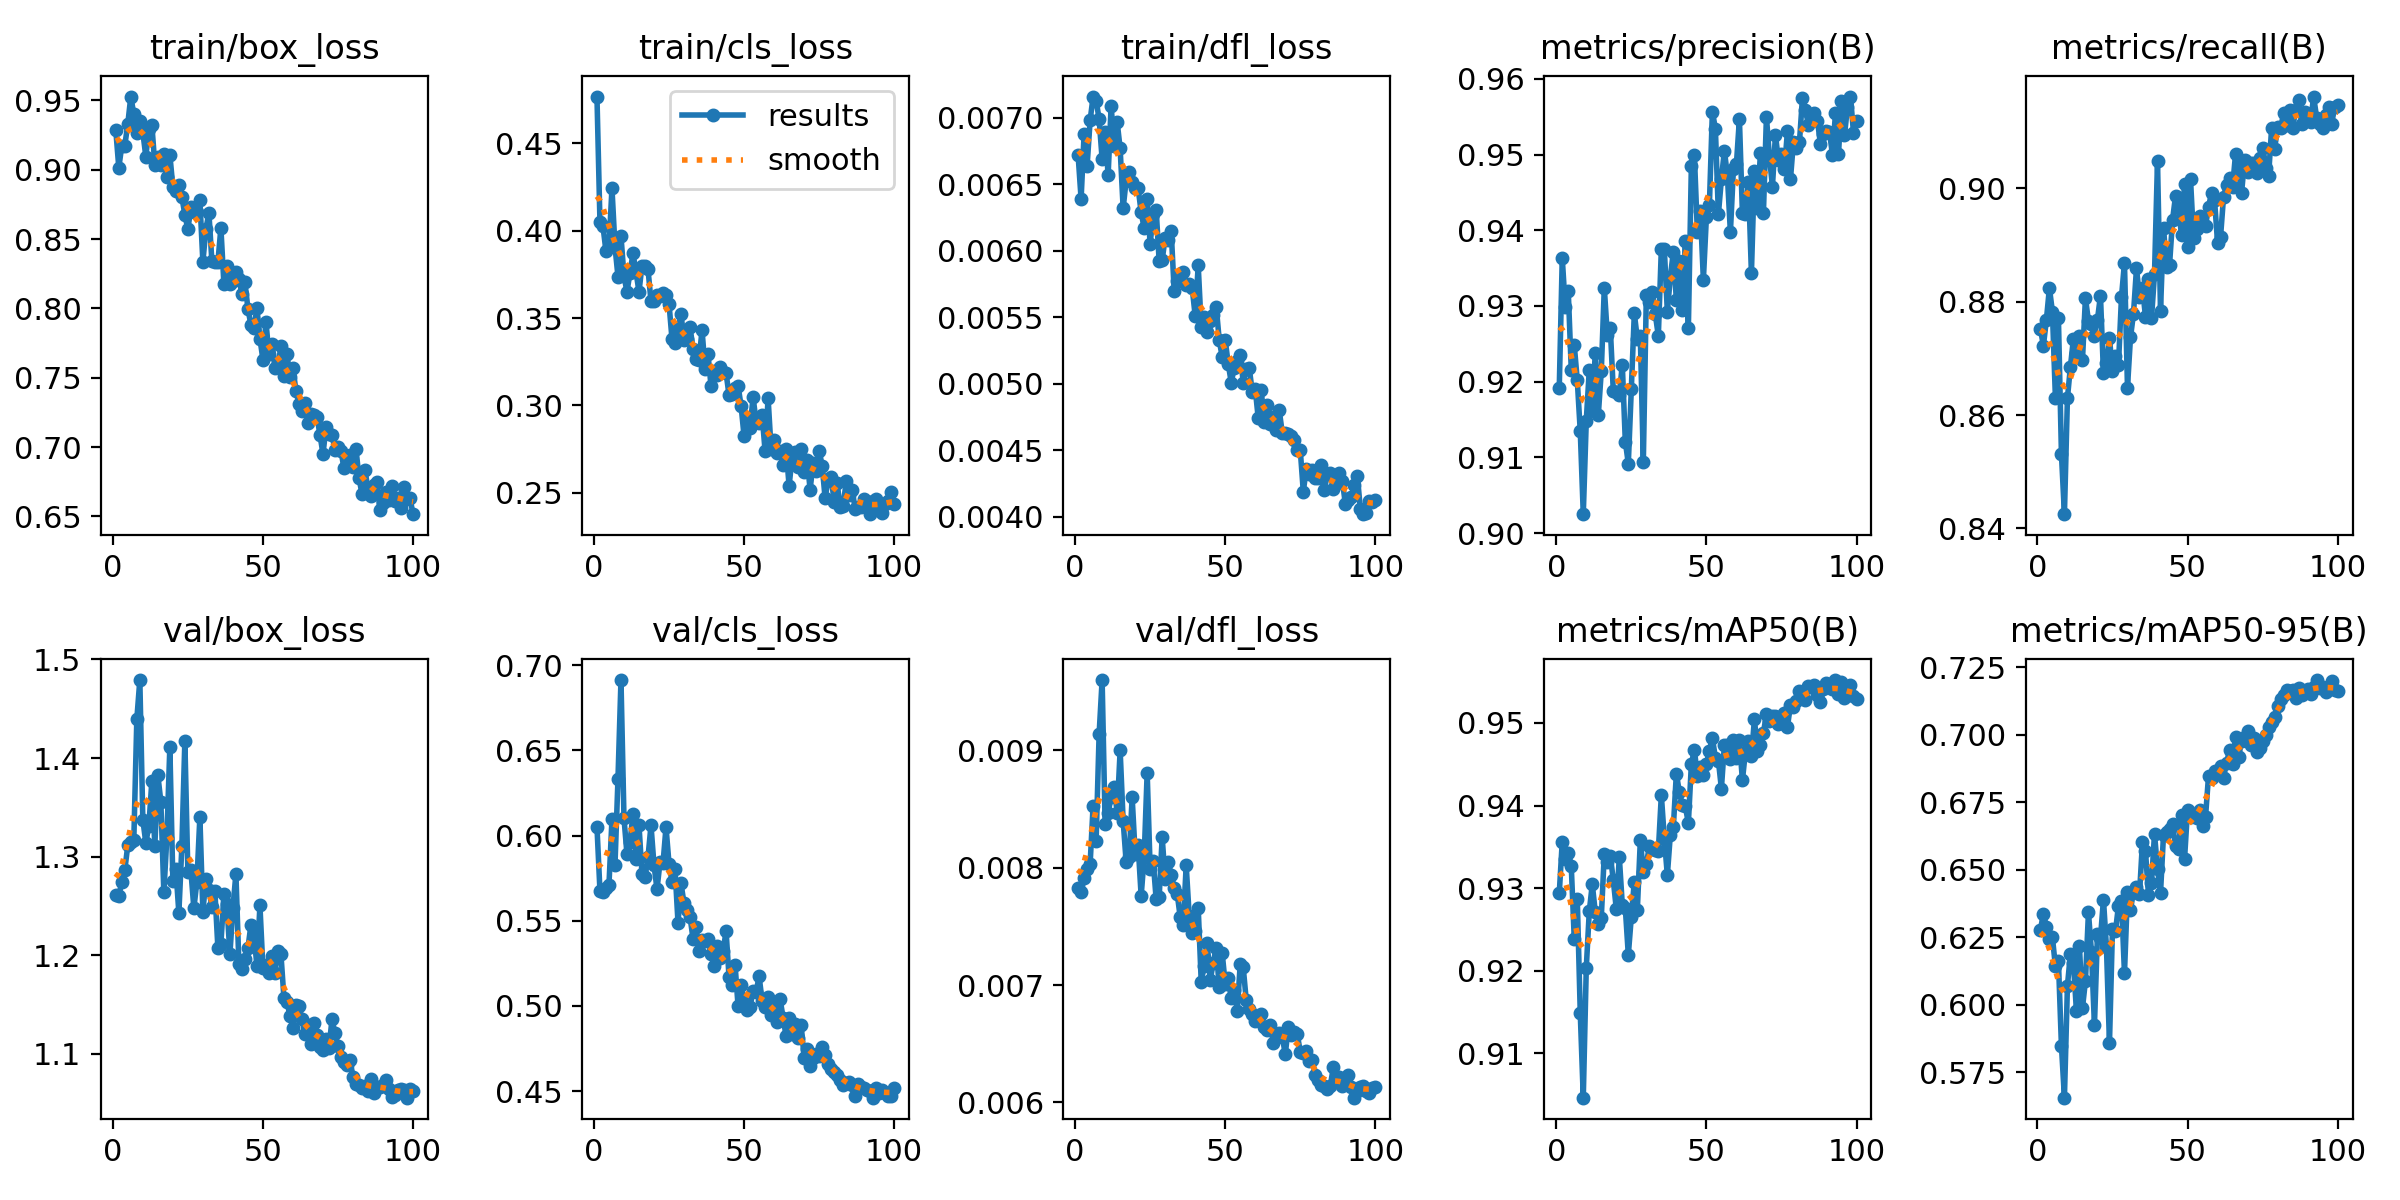
\includegraphics[width=\textwidth]{results_train78.png}
    \caption{Stage~II (train78, 100 epochs)}
  \end{subfigure}
  \hfill
  \begin{subfigure}[t]{0.48\textwidth}
    \centering
    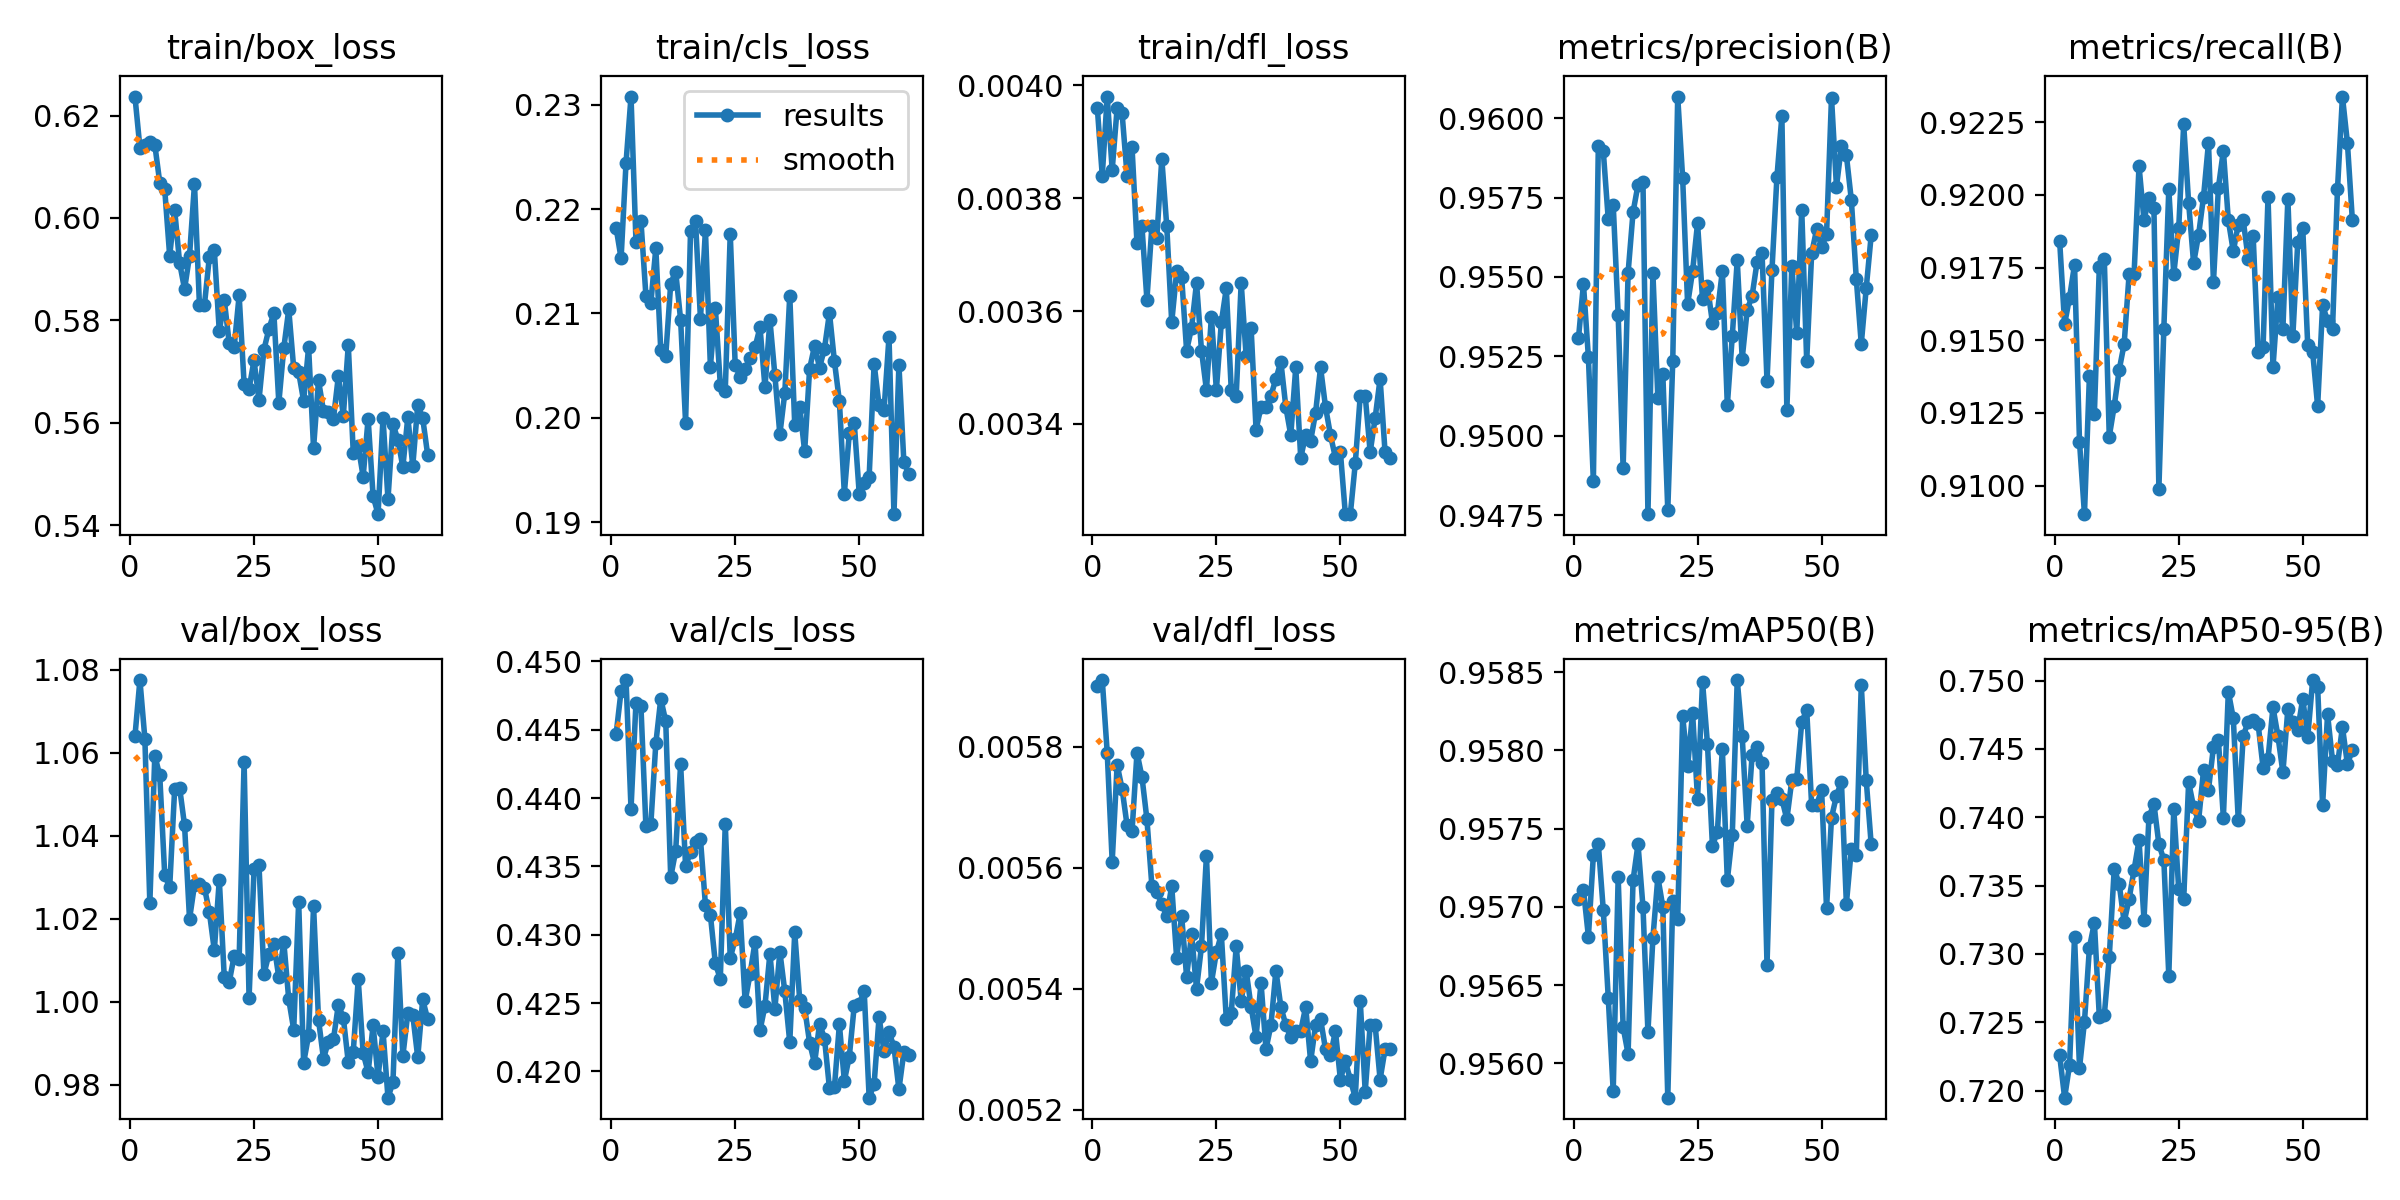
\includegraphics[width=\textwidth]{results_train81.png}
    \caption{Stage~III (train81, 60 epochs)}
  \end{subfigure}

  \caption{Ultralytics auto-generated training result plots for each
    stage, showing train/val losses, precision, recall, and mAP metrics.}
  \label{fig:ultralytics_plots}
\end{figure}

% ──────────────────────── Bibliography ────────────────────────────
\begin{thebibliography}{9}

  \bibitem{ultralytics2025yolo}
  Ultralytics,
  ``Ultralytics YOLO: Real-Time Object Detection,'' 2025.
  \url{https://github.com/ultralytics/ultralytics}

  \bibitem{lin2014coco}
  T.-Y.~Lin, M.~Maire, S.~Belongie, et~al.,
  ``Microsoft COCO: Common Objects in Context,''
  in \emph{European Conference on Computer Vision (ECCV)},
  pp.~740--755, Springer, 2014.

  \bibitem{buslaev2020albumentations}
  A.~Buslaev, V.~I.~Iglovikov, E.~Khvedchenya, A.~Parinov,
  M.~Druzhinin, and A.~A.~Kalinin,
  ``Albumentations: Fast and Flexible Image Augmentations,''
  \emph{Information}, vol.~11, no.~2, p.~125, 2020.

  \bibitem{bochkovskiy2020yolov4}
  A.~Bochkovskiy, C.-Y.~Wang, and H.-Y.~M.~Liao,
  ``YOLOv4: Optimal Speed and Accuracy of Object Detection,''
  \emph{arXiv preprint arXiv:2004.10934}, 2020.

  \bibitem{loshchilov2016sgdr}
  I.~Loshchilov and F.~Hutter,
  ``SGDR: Stochastic Gradient Descent with Warm Restarts,''
  \emph{arXiv preprint arXiv:1608.03983}, 2016.

\end{thebibliography}

\end{document}
